\documentclass[a4paper,12pt]{report}

\usepackage{alltt, fancyvrb, url}
\usepackage{graphicx}
\usepackage{subfigure}
\usepackage{array}
\usepackage{wrapfig}
\usepackage{algorithmic}
\usepackage[utf8]{inputenc}
\usepackage{fontenc}
\usepackage{amsmath,stmaryrd,mathtools,algorithm}
\usepackage{amssymb}
\usepackage{float}
\usepackage{hyperref}
\usepackage[table]{xcolor}
\usepackage{adjustbox}
\usepackage{setspace}


\begin{document}

    
	\title{Elaborato per il corso di Basi di dati}
	\author{
      Davide Carità - 0000873616\\
      \texttt{davide.carita@studio.unibo.it}
      \and
      Pietro Olivi - 0001020332\\
      \texttt{pietro.olivi2@studio.unibo.it}
      \and
      Lorenzo Dalmonte - 0001021552\\
      \texttt{lorenzo.dalmonte4@studio.unibo.it}
    }
	\date{}
	
    \maketitle
	\tableofcontents*
	\newpage

	\chapter{Analisi dei requisiti}

        \section{Requisiti in linguaggio naturale}
    	
        Si vuole realizzare una base di dati che supporti le funzionalità di un' applicazione di compravendita di immobili nonché il monitoraggio del welfare delle principali città europee. All'interno dell'applicazione, si potrà creare un account che permetta agli utenti di promuovere e vendere le loro proprietà attraverso la piattaforma. Allo stesso tempo, gli utenti potranno utilizzare l'applicazione per cercare e visualizzare annunci immobiliari disponibili. \\ \\ Uno dei servizi sarà quello di individuare la città europea che meglio si adatta alle proprie esigenze: si potrà vedere ad esempio quale città ha ottenuto i migliori punteggi a livello europeo in tema di qualità dell'aria, costo della vita o efficienza sanitaria. Oltre a ciò, saranno disponibili anche i dati relativi agli anni precedenti, in modo da avere uno storico che permetta di valutare lo sviluppo del welfare nella città selezionata. 
        Una volta che gli utenti hanno individuato la propria città ideale, il servizio offrirà la possibilità di visualizzare annunci immobiliari specifici suddivisi per diverse zone all'interno della città. 
        Questa suddivisione permette agli utenti di esplorare le opzioni abitative in aree specifiche che potrebbero essere più in linea con le loro preferenze e esigenze. \\ \\ Gli annunci immobiliari saranno suddivisi in tre tipi: vendita, affitto e asta, e forniranno dettagli completi sugli immobili, compresi la metratura, il numero di stanze, il prezzo e altre informazioni pertinenti. Oltre a ciò, il servizio fornirà la funzionalità di avviare una conversazione tra acquirente e venditore, offrendo loro la possibilità di scambiarsi informazioni in modo rapido. Sarà data la possibilità ai giudici d'esecuzione di creare un account privilegiato che consentirà loro di gestire delle aste immobiliari. Questo account fornirà ai giudici strumenti e funzionalità speciali per gestire l'intero processo di vendita all'asta, inclusa la creazione e la pubblicazione degli annunci, la gestione delle offerte e altre attività correlate.

    	\section{Estrazione dei concetti principali}

        {\Large \textbf{Città}} $\rightarrow$ Le città sono suddivise in diverse zone e vengono valutate in base a parametri di welfare. Gli utenti utilizzano l'applicazione per individuare la città che meglio si adatta alle loro esigenze e preferenze abitative. \\
        \\
        {\Large \textbf{Categoria}} $\rightarrow$ Le categorie di welfare sono criteri utilizzati per valutare il benessere nelle città europee. Essi includono ambiente, trasporto, economia, sanità ed istruzione. Questi parametri forniscono un quadro del livello di comfort e salute delle città. Consentono agli utenti di confrontare le città in base a questi indicatori, facilitando la scelta di una città che meglio si adatta alle proprie esigenze.
            \begin{itemize}
                \item \textbf{Ambiente}
                            Valuta la qualità ambientale delle città, con indicatori come il pm 2.5 (particolato fine) e la percentuale di spazio verde urbano.
                \item \textbf{Trasporto} 
                            Valuta l'efficienza dei sistemi di trasporto urbano, considerando il tempo medio di pendolarismo e il numero di auto per persona.
                \item \textbf{Economia} 
                            Valuta la vitalità economica di una città attraverso indicatori come il PIL pro capite, lo stipendio medio e il tasso di disoccupazione. Consente inoltre di avere un'indicazione sul livello di prosperità e opportunità lavorative presenti nell'area urbana considerata.
                \item \textbf{Sanità}
                            Valuta la qualità del sistema sanitario di una città, considerando l'aspettativa di vita e il numero di posti letto, all'interno degli ospedali, per abitante. Fornisce un'indicazione sulla salute generale e sull'accessibilità alle cure mediche
                \item \textbf{Istruzione} 
                            Valuta la qualità dell'istruzione in una città, considerando la percentuale di laureati, la percentuale di diplomati e il numero di università presenti oltre che dare un'indicazione sulla disponibilità e l'accessibilità all'istruzione superiore e alla formazione professionale nell'area urbana considerata.
                \end{itemize} 
        {\Large \textbf{Immobile}} $\rightarrow$ Un immobile si riferisce a una proprietà che può essere venduta, affittata o messa all'asta dagli utenti attraverso la piattaforma. Gli annunci immobiliari includono informazioni come la metratura, il numero di stanze, il prezzo e altre caratteristiche rilevanti dell'immobile. \\
        \\
        {\Large \textbf{Annuncio}} $\rightarrow$ Una presentazione di un immobile disponibile per la vendita, l'affitto o l'asta. Gli annunci forniscono dettagli completi sull'immobile, come la sua ubicazione, le specifiche, i prezzi e altre informazioni pertinenti. Gli utenti utilizzano l'applicazione per cercare, visualizzare e interagire con gli annunci immobiliari. \\
        \\
        {\Large \textbf{Account}} $\rightarrow$ Gli utilizzatori possono creare un account utente per promuovere e vendere le loro proprietà, cercare annunci immobiliari disponibili, avviare conversazioni con acquirenti o venditori e gestire altre attività correlate. Ai giudici d'esecuzione viene fornita la possibilità di creare un account privilegiato con strumenti e funzionalità speciali per gestire le aste immobiliari e le attività associate al processo di vendita all'asta. \\
        \\
        \textbf{Di seguito le principali azioni richieste:}
        
        \begin{enumerate}
        \item Creare un account utente.
        \item Pubblicare un annuncio immobiliare di vendita/affitto/asta.
        \item Visualizzare annunci immobiliari disponibili.
        \item Mostrare dettagli completi di un immobile.
        \item Avviare una conversazione con un venditore.
        \item Visualizzare punteggi di welfare di una città.
        \item Filtrare annunci immobiliari per criteri (es. prezzo, dimensioni).
        \end{enumerate}


	\chapter{Progettazione concettuale}
        La progettazione concettuale, derivata dall'analisi dei concetti principali del dominio,
        è stata incrementale in termini di complessità. Di seguito passeremo quindi in rassegna
        gli stadi dello schema cronologicamente ordinati, illustrando le motivazioni che hanno 
        portato ad effettuare i vari raffinamenti. 

        \section{Schema scheletro}
        Il primo schema è il risultato della trasposizione su E/R delle astrazioni formulate nel capitolo precedente.
        In primo piano figura l'entita \textit{città}, caratterizzata da al più N \textit{valutazioni} generiche,
        ciascuna delle quali espressa con un punteggio intero nell'intervallo [0,10]. \\
        \\
        La città è identificata da un codice univoco, in modo da evitare di incappare in uno dei ricorrenti scenari di 
        città omonime nella medesima nazione (dove lo stato ed il nome della città non sarebbero sufficienti a distinguerle). Sebbene in molti casi ciò possa essere risolto specificando la regione di appartenenza 
        delle città "doppione", rimarrebbero comunque insolute casistiche tipiche del territorio britannico, dove città omonime 
        potrebbero situarsi in contee diverse ma all'interno della stessa "Government Office \textit{Region}". A titolo di esempio, basti
        pensare che nell'intero UK compaiono 14 città chiamate Newport! \footnote{https://www.southwalesargus.co.uk/news/19433701.newports-across-world/} \\
        \\
        Un annuncio riguarda un solo immobile, mentre lo stesso immobile può comparire in più annunci diversi. Quest'ultima cardinalità,
        meno ovvia, deriva dall'esigenza di conservare lo storico di tutte le vendite/affitti di ciascuna abitazione, in modo da formulare
        in seguito un trend del prezzo in funzione del tempo (da presentare agli interessati).

        \begin{figure}[ht]
            \centering{}
            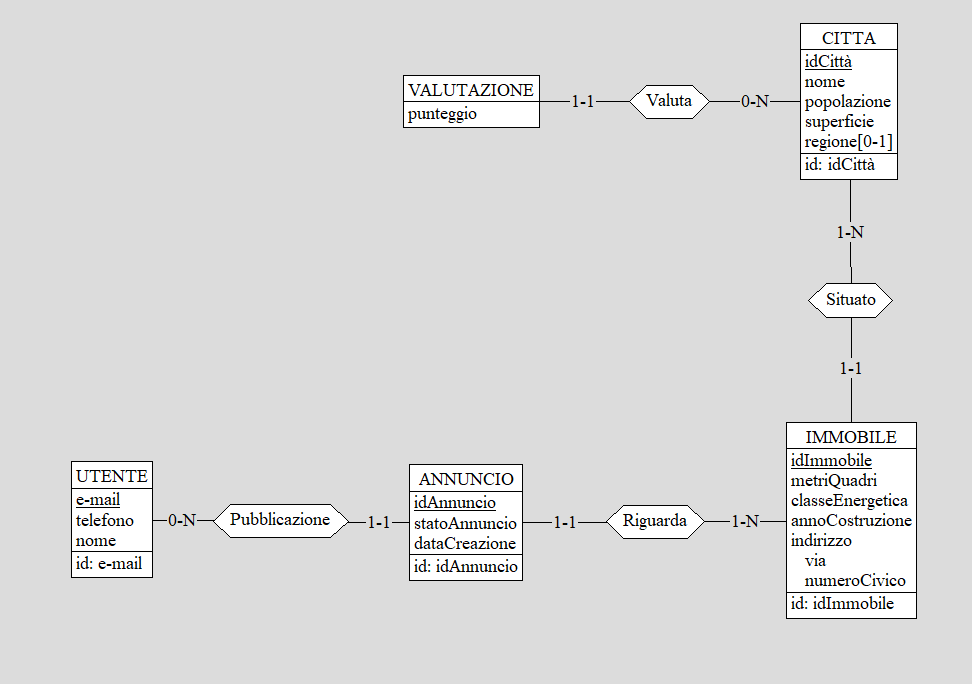
\includegraphics[width=\linewidth]{./images/first.png}
            \caption{La prima versione dello schema concettuale}
        \end{figure}

        \section{Divisione in zone e di immobili}
        Introducendo una gerarchia per differenziare le varie tipologie di \textit{immobili} inserite negli annunci,
        ogni immobile dovrà essere necessariamente contraddistinto da un ID proprio. Perchè? Se tutte le dimore
        fossero case indipendenti, allora potrebbero essere identificate da attributi che ne specifichino la posizione.
        Aggiungendo gli appartamenti poi, basterebbe includere nella chiave un campo che indichi il numero dell'interno.
        Con l'avvento delle stanze singole tuttavia, la soluzione precedentemente adottata risulterà inadatta, poichè 
        non risponderebbe alla necessità di un utente di affittare più stanze della stessa abitazione (ognuna con un 
        annuncio dedicato).

        \begin{figure}[ht]
            \centering{}
            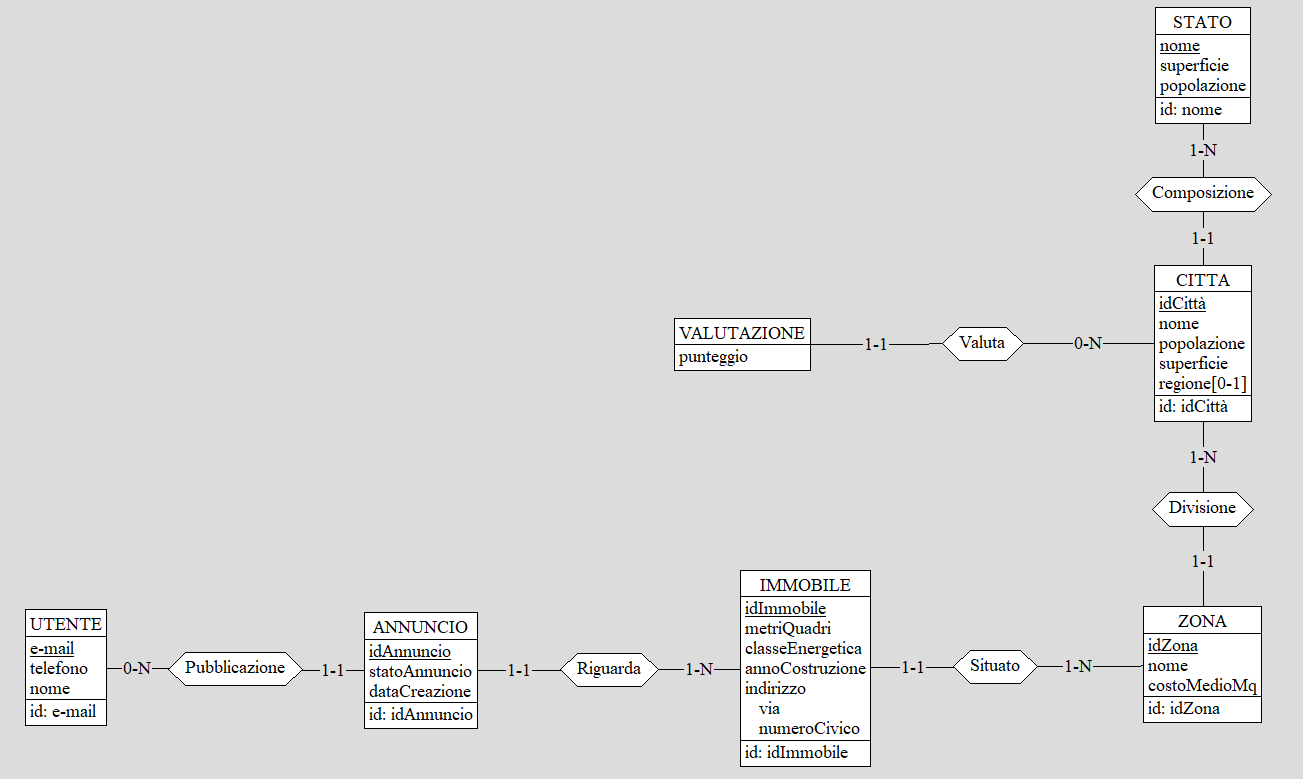
\includegraphics[width=\linewidth]{./images/second.png}
            \caption{La seconda versione dello schema concettuale}
        \end{figure}

        \section{Espansione delle valutazioni}
        Nell’amplificazione della porzione di schema relativa all’analisi delle città abbiamo scisso la precedente entità 
        “segnaposto” \textit{valutazione} in una serie di categorie, come illustrato nei requisiti. Ciascuna di queste è caratterizzata 
        da parametri dal dominio numerico (e.g. \textit{ambiente} da \textit{PM2.5media} e \textit{percentualeSpazioVerdeUrbano}), in
        base ai cui valori verrà calcolato in automatico un punteggio onnicomprensivo per la categoria, poi conservato nel campo 
        corrispondente di \textit{città\textunderscore anno} (\textit{punteggioAmbiente} nell’esempio citato). \\
        \\
        Il ruolo dell’entità \textit{città\_anno} è quello di consentire la storicizzazione dei punteggi ottenuti da ciascuna città 
        negli anni passati, in modo da poter computare lo sviluppo, o l’involuzione, a cui il luogo ha assistito. Ciascuna istanza 
        di categoria può far riferimento a più città ed in più anni diversi: Parigi e Londra potrebbero aver registrato stessi 
        \textit{PILProCapite, stipendioMedio e tassoDisoccupazione} nel 2019, così come Heidelberg potrebbe aver riconfermato gli 
        stessi valori relativi alla \textit{sanità} dell'anno precedente. Ad ogni \textit{città\_anno}, invece, è collegata una ed 
        una sola istanza di tutte le 5 categorie. \\
        \\
        
        \begin{figure}[ht]
            \centering{}
            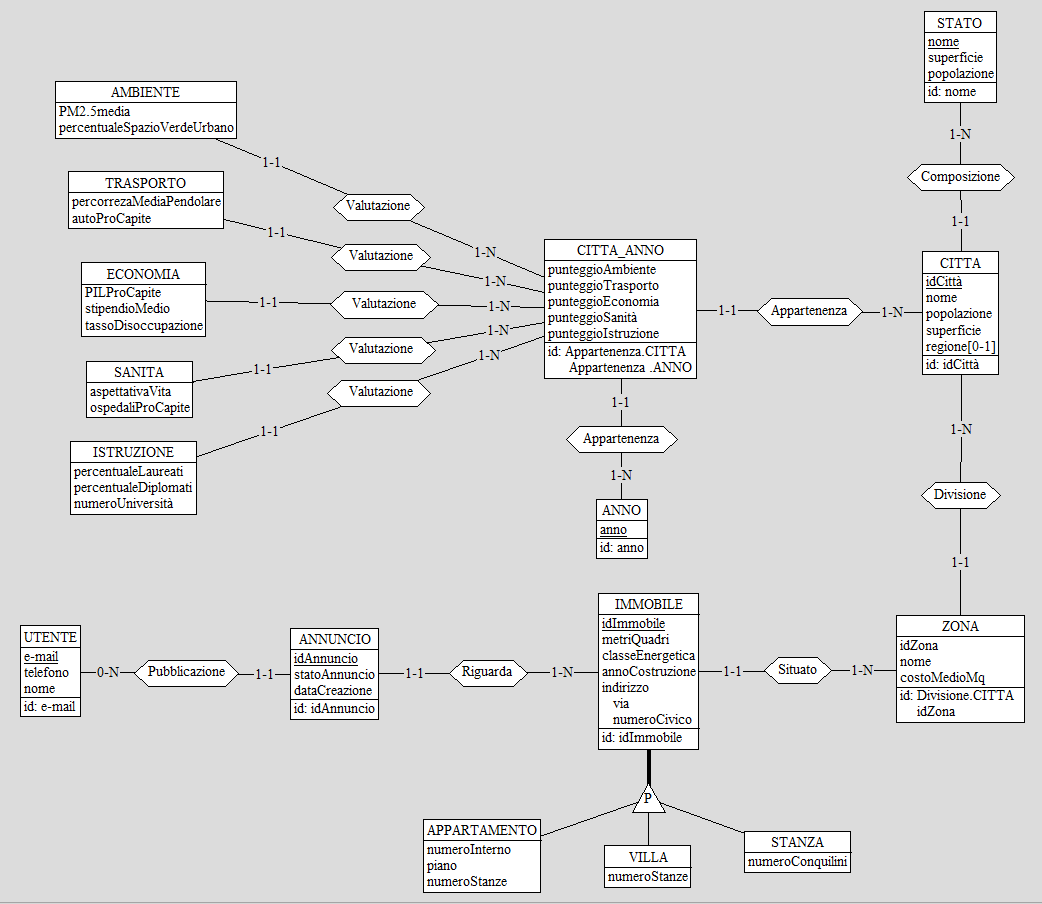
\includegraphics[width=\linewidth]{./images/third.png}
            \caption{La terza versione dello schema concettuale}
        \end{figure}

        \section{Aste e giudici}
        Per enfatizzare la differente natura degli annunci pubblicabili dagli utenti ordinari e le aste riservate ad i giudici,
        si è deciso di scindere l'entità \textit{annuncio} rispettivamente in \textit{annuncio\_utente} ed \textit{asta}. \\
        \\
        Le aste sono tipologie di annunci la cui gestione (dunque pubblicazione) è riservata ad i giudici di esecuzione.
        In particolare, ciascuna asta verrà amministrata da uno ed un solo giudice, il quale però potrà dirigerne fino ad N.
        Per riprodurre le dinamiche di ascesa del prezzo ed infine di vendita, viene istituita l’entità rialzo. \\
        \\
        Durante il periodo di attività di un’asta, scandito da una data di inizio ed una di fine, gli utenti hanno la facoltà di avanzare più rialzi 
        (Il collegare direttamente utente ad asta avrebbe ristretto il numero massimo di rialzi effettuabili da un utente, nella stessa asta, ad 1).
        I rialzi ricevuti in una determinata asta sono identificati univocamente dall’ utente che li ha effettuati e l’istante temporale in cui sono 
        stati offerti. Al termine di un asta, si può risalire al prezzo di vendita, ove avvenuta, verificando il rialzo più recente ad essa collegato.
        	
    	\section{Introduzione della messaggistica}
        La messaggistica viene modellata attraverso le associazioni tra le entità \textit{utente $\Leftrightarrow$ messaggio} e 
        \textit{messaggio $\Leftrightarrow$ annuncio\_utente}. In prima battuta ci si potrebbe erroneamente domandare il motivo 
        del non aver optato per una relazione ad anello tra \textit{utenti}, con il testo del messaggio racchiuso in un campo 
        dell’ associazione, tuttavia tale configurazione consentirebbe di memorizzare nella base di dati al più un 
        \textit{messaggio} per ogni coppia di utenti! \\
        \\
        Sarebbe inoltre fuorviante collegare ogni messaggio direttamente 
        a mittente e destinatario poiché non si terrebbe conto del caso in cui le stesse due persone dovessero contattarsi in merito ad annunci 
        diversi, anche contemporaneamente, e non si riuscirebbe dunque a dedurre il contesto dei messaggi. Per risolvere quest’ultima problematica 
        si è deciso di interporre l'enitità \textit{messaggio} tra \textit{utente}, nonchè il potenziale acquirente, ed \textit{annuncio\_utente}, 
        ossia il gestore dell’inserzione nelle vesti del suo annuncio. I messaggi all’interno di ogni chat vengono identificati dall’istante 
        temporale in cui sono inviati (timestamp). \\
        



        \begin{figure}[ht]
            \centering{}
            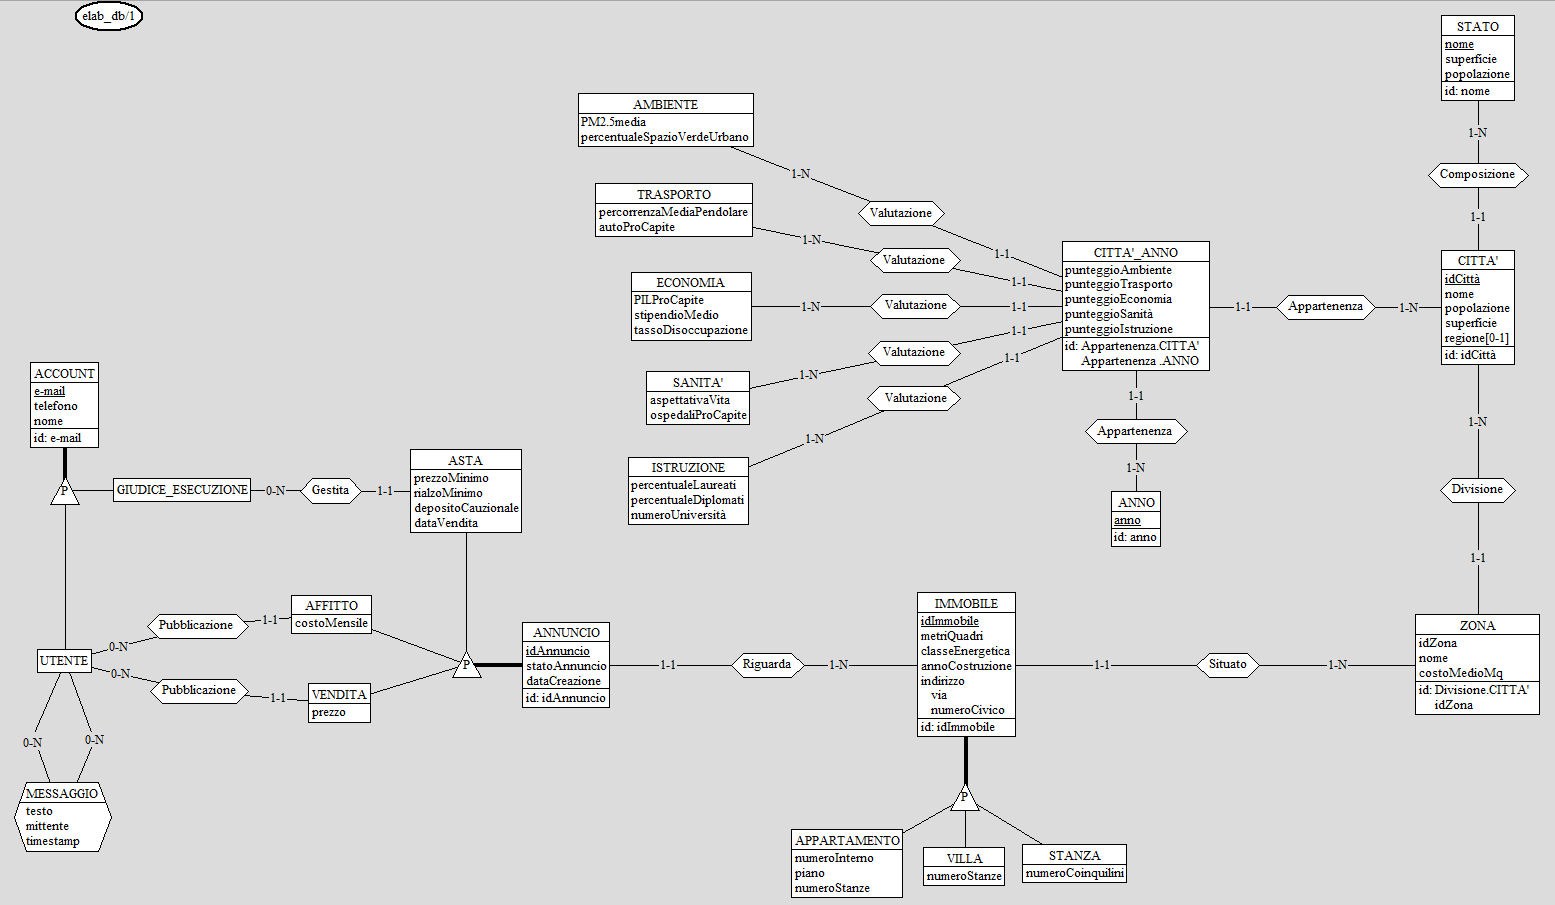
\includegraphics[width=\linewidth]{./images/fourth.png}
            \caption{L'ultima versione dello schema concettuale}
        \end{figure}

        	
	\chapter{Progettazione logica} 
    \definecolor{LightCyan}{rgb}{0.88,1,1}

    	\section{Stima del volume dei dati}
        \begin{table}[H]
            \centering
             \begin{tabular}{lcr}
             \rowcolor{LightCyan}\textbf{Concetto} & \textbf{Costrutto} & \textbf{Volume} \\ [0.5ex] 
             \hline
             Stato & E & 50 \\
             Composizione & R & 700 \\ 
             Città & E & 700 \\
             Divisione & R & 7.000 \\
             Zona & E & 7.000 \\
             Città\_Anno & E & 14.000 \\
             Appartenenza & R & 14.000 \\
             Riferimento & R & 14.000 \\ 
             Anno & E & 20 \\
             Ambiente & E & 12.000 \\
             Valutazione\_A & R & 12.000 \\
             Trasporto & E & 12.000 \\
             Valutazione\_T & R & 12.000 \\
             Economia & E & 12.000 \\
             Valutazione\_E & R & 12.000 \\
             Sanità & E & 12.000 \\
             Valutazione\_S & R & 12.000 \\
             Istruzione & E & 12.000 \\
             Valutazione\_I & R & 12.000 \\ [1ex] 
             
             \end{tabular}
        \end{table}

        \begin{table}[H]
            \centering
             \begin{tabular}{lcr} 
             \rowcolor{LightCyan} \textbf{Concetto} & \textbf{Costrutto} & \textbf{Volume} \\ [0.5ex] 
             \hline
             Situato & R & 350.000 \\
             Immobile & E & 350.000 \\
             Appartamento & E & 116.700 \\ 
             Villa & E & 116.700 \\
             Stanza & E & 116.700 \\
             Riguarda & R & 450.000 \\
             Annuncio & E & 450.000 \\
             Asta & E & 50.000 \\
             Annuncio\_Utente & E & 400.000 \\ 
             Affitto & E & 200.000 \\
             Vendita & E & 200.000 \\
             Invio/Ricezione & R & 15.000.000 \\
             Ricezione/Invio & R & 15.000.000 \\
             Messaggio & E & 15.000.000 \\
             Pubblicazione & R & 400.000 \\
             Account & E & 1.505.000 \\ 
             Utente & E & 1.500.000 \\
             Offerta & R & 750.000 \\
             Rialzo & E & 750.000 \\ 
             Accoglimento & R & 750.000 \\ 
             Gestione & R & 50.000 \\ 
             Giudice\_Esecuzione & E & 5.000 \\ [1ex] 
             \end{tabular}
        \end{table}


    	\section{Descrizione delle operazioni principali e stima della loro frequenza}
        \begin{table}[H]
            \centering
            \begin{adjustbox}{width=1.45\textwidth,center}
            \begin{tabular}{clr}
            \rowcolor{LightCyan} \textbf{Codice} & \textbf{Operazione} & \textbf{Frequenza} \\ [0.5ex] 
            \hline
             1 & Registrare un nuovo account & 1.500 al giorno \\
             2 & Pubblicare un annuncio immobiliare (vendita, affitto o asta) & 500 al giorno \\
             3 & Visualizzare annunci immobiliari attivi di una città in ordine cronologico & 50.000 al giorno \\ 
             4 & Suddividere gli annunci in vendita, affitto o asta all'interno di una città & 35.000 al giorno \\
             5 & Ordinare gli immobili in base a particolari filtri (e.g. metratura, classe energetica) & 5.000 al giorno \\
             6 & Filtrare gli annunci per zona & 40.000 al giorno \\
             7 & Ordinare gli annunci di affitto per costo mensile & 12.000 al giorno \\
             8 & Mostrare aste attive in una città & 7.500 al giorno \\
             9 & Ordinare le aste per prezzo attuale crescente & 4.000 al giorno \\ 
             10 & Effettuare un rialzo all'interno di un'asta (controllando la sua validità) & 500 al giorno \\
             11 & Contattare un utente in merito ad un annuncio creato & 15.000 al giorno \\
             12 & Ricostruire una conversazione tra due utenti & 30.000 al giorno \\
             13 & Andamento del prezzo di un immobile in funzione del tempo & 5.000 al giorno \\
             14 & Comparare il prezzo di un immobile al mq con quello degli immobili nella stessa zona & 10.000 al giorno \\
             15 & Comparare il prezzo di un immobile al mq con quello degli immobili nella stessa città & 7.500 al giorno \\
             16 & Comparare il prezzo medio al mq di una zona con quello della città & 3.500 al giorno \\ 
             17 & Ordinare le zone di una città per costo medio al mq & 1.500 al giorno \\
             18 & Stilare una top 5 città per una o più categorie & 3.000 al giorno \\
             19 & Classificare città in base all'evoluzione in una o più categorie rispetto all'anno precedente & 500 al giorno \\ 
             20 & Ordinare le città in base a valori specifici di una o più categorie & 1.000 al giorno \\ 
             21 & Calcolare performance di uno stato in una o più categorie (da ogni città) & 2.000 al giorno \\ 
             22 & Aggiornamento annuale dei punteggi di una città (dati i campi delle categorie) & 1 all'anno \\ [1ex]
            \end{tabular}
            \end{adjustbox}
            \end{table}
        	
    	\section{Schemi di navigazione e tabelle degli accessi}	

        \textbf{OP 1: Registrare un nuovo account}
        	\begin{table}[H]
            \centering
             \begin{tabular}{llll}
             \rowcolor{yellow!20}\textbf{Concetto} & \textbf{Costrutto} & \textbf{Accessi} & \textbf{Tipo} \\ [0.5ex] 
             \hline
             Account & E & 1 & Scrittura \\ 
             \hline
             \rowcolor{yellow!20}\rowcolor{yellow!20} &   & \textbf{Totale:} 1S $\rightarrow$ 3.000 al giorno &  \\ [1ex] 
             \end{tabular}
            \end{table}

            \textbf{OP 2: Pubblicare un annuncio immobiliare (vendita, affitto o asta)}
            Viene di seguito presentato il caso in cui si voglia aggiungere un annuncio relativo ad un immobile
            non ancora presente nella base di dati: sarà necessario aggiornare, dunque riscrivere, i campi 
            \textit{numeroImmobili} e \textit{costoMedioMq}.
        	\begin{table}[H]
            \centering
             \begin{tabular}{llll}
             \rowcolor{yellow!20} \textbf{Concetto} & \textbf{Costrutto} & \textbf{Accessi} & \textbf{Tipo} \\ [0.5ex] 
             \hline
             Annuncio & E & 1 & Scrittura \\ 
             Riguarda & R & 1 & Scrittura \\ 
             Immobile & E & 1 & Scrittura \\ 
             Situato & R & 1 & Scrittura \\ 
             Zona & E & 1 & Scrittura \\ 
             \hline
             \rowcolor{yellow!20}  \rowcolor{yellow!20} &   & \textbf{Totale:} 5S $\rightarrow$ 5.000 al giorno &  \\ [1ex] 
             \end{tabular}
            \end{table} 
            Nell'eventualità in cui venisse pubblicato un'annuncio relativo ad un immobile già comparso sulla
            piattaforma, e pertanto già considerato nel calcolo del \textit{costoMedioMq} del quartiere di
            appartenenza, dovremmo leggere il prezzo al mq designato dal proprietario più recente rispetto all'attuale, 
            sottrarlo a costoMedioMq*numeroImmobili, aggiungere il nuovo e ri-dividere per lo stesso numeroImmobili.
            
        	\begin{table}[H]
            \centering
             \begin{tabular}{llll}
             \rowcolor{yellow!20}\rowcolor{yellow!20} \textbf{Concetto} & \textbf{Costrutto} & \textbf{Accessi} & \textbf{Tipo}\\ [0.5ex] 
             \hline
             Annuncio & E & 1 & Lettura \\
             Annuncio & E & 1 & Scrittura \\
             Riguarda & R & 1 & Scrittura \\ 
             Immobile & E & 1 & Lettura \\ 
             Situato & R & 1 & Lettura \\ 
             Zona & E & 1 & Scrittura \\  
             \hline
             \rowcolor{yellow!20} &   & \textbf{Totale:} 3L + 3S $\rightarrow$ 1.800 al giorno &  \\ [1ex] 
             \end{tabular}
            \end{table}

            \textbf{OP 3: Visualizzare annunci immobiliari attivi di una città in ordine cronologico} \\
            Data una città, prendiamo le sue 10 zone, che hanno in media 5 immobili l'una. Visto che gli annunci totali \textit{attivi} (worst case 450.000) 
            sono $\ge$ degli immobili (350.000) (considerando che lo stesso immobile può essere pubblicato sia come affitto che vendita)
            uso lo stesso loro rapporto (1,3) per calcolare le letture che farò negli annunci.
        	\begin{table}[H]
            \centering
             \begin{tabular}{llll}
             \rowcolor{yellow!20} \textbf{Concetto} & \textbf{Costrutto} & \textbf{Accessi} & \textbf{Tipo}\\ [0.5ex] 
             \hline
             Città & E & 1 & Lettura \\ 
             Divisione & R & 10 & Lettura \\ 
             Zona & E & 10 & Lettura \\ 
             Situato & R & 50 & Lettura \\ 
             Immobile & E & 50 & Lettura \\ 
             Riguarda & R & 65 & Lettura \\ 
             Annuncio & E & 65 & Lettura \\ 
             \hline
                \rowcolor{yellow!20} &   & \textbf{Totale:} 251L $\rightarrow$ 12.550.000 al giorno &  \\ [1ex] 
             
             \end{tabular}
            \end{table}

            \textbf{OP 4: Suddividere gli annunci in vendita, affitto o asta all’interno di una città}
        	\begin{table}[H]
            \centering
             \begin{tabular}{llll}
             \rowcolor{yellow!20} \textbf{Concetto} & \textbf{Costrutto} & \textbf{Accessi} & \textbf{Tipo}\\ [0.5ex] 
             \hline
             Città & E & 1 & Lettura \\ 
             Divisione & R & 10 & Lettura \\ 
             Zona & E & 10 & Lettura \\ 
             Situato & R & 50 & Lettura \\ 
             Immobile & E & 50 & Lettura \\ 
             Riguarda & R & 65 & Lettura \\ 
             Annuncio & E & 65 & Lettura \\ 
             \hline
                \rowcolor{yellow!20} &   & \textbf{Totale:} 251L $\rightarrow$ 8.785.000 al giorno &  \\ [1ex] 
             
             \end{tabular}
            \end{table}

            \textbf{OP 5: Ordinare gli annunci in base a particolari filtri sull'immobile (e.g. metratura, classe energetica)}
        	\begin{table}[H]
            \centering
             \begin{tabular}{llll}
             \rowcolor{yellow!20} \textbf{Concetto} & \textbf{Costrutto} & \textbf{Accessi} & \textbf{Tipo}\\ [0.5ex] 
             \hline
             Città & E & 1 & Lettura \\ 
             Divisione & R & 10 & Lettura \\ 
             Zona & E & 10 & Lettura \\ 
             Situato & R & 50 & Lettura \\ 
             Immobile & E & 50 & Lettura \\
             Riguarda & R & 65 & Lettura \\ 
             Annuncio & E & 65 & Lettura \\ 
             \hline
                \rowcolor{yellow!20} &   & \textbf{Totale:} 251L $\rightarrow$ 1.255.000 al giorno &  \\ [1ex] 
             
             \end{tabular}
            \end{table}

            \textbf{OP 6: Filtrare gli annunci per zona}
        	\begin{table}[H]
            \centering
             \begin{tabular}{llll}
             \rowcolor{yellow!20} \textbf{Concetto} & \textbf{Costrutto} & \textbf{Accessi} & \textbf{Tipo}\\ [0.5ex] 
             \hline
             Città & E & 1 & Lettura \\ 
             Divisione & R & 10 & Lettura \\ 
             Zona & E & 10 & Lettura \\ 
             Situato & R & 50 & Lettura \\ 
             Immobile & E & 50 & Lettura \\
             Riguarda & R & 65 & Lettura \\ 
             Annuncio & E & 65 & Lettura \\ 
             \hline
                \rowcolor{yellow!20} &   & \textbf{Totale:} 251L $\rightarrow$ 10.040.000 al giorno &  \\ [1ex] 
             
             \end{tabular}
            \end{table}

            \textbf{OP 7: Ordinare gli annunci di affitto per costo mensile}
        	\begin{table}[H]
            \centering
             \begin{tabular}{llll}
             \rowcolor{yellow!20} \textbf{Concetto} & \textbf{Costrutto} & \textbf{Accessi} & \textbf{Tipo}\\ [0.5ex] 
             \hline
             Città & E & 1 & Lettura \\ 
             Divisione & R & 10 & Lettura \\ 
             Zona & E & 10 & Lettura \\ 
             Situato & R & 50 & Lettura \\ 
             Immobile & E & 50 & Lettura \\ 
             Riguarda & R & 65 & Lettura \\ 
             Annuncio & E & 65 & Lettura \\ 
             \hline
                \rowcolor{yellow!20} &   & \textbf{Totale:} 251L $\rightarrow$ 3.012.000 al giorno &  \\ [1ex] 
             
             \end{tabular}
            \end{table}

            \textbf{OP 8: Mostrare aste attive in una città}
        	\begin{table}[H]
            \centering
             \begin{tabular}{llll}
             \rowcolor{yellow!20} \textbf{Concetto} & \textbf{Costrutto} & \textbf{Accessi} & \textbf{Tipo}\\ [0.5ex] 
             \hline
             Città & E & 1 & Lettura \\ 
             Divisione & R & 10 & Lettura \\ 
             Zona & E & 10 & Lettura \\ 
             Situato & R & 50 & Lettura \\ 
             Immobile & E & 50 & Lettura \\ 
             Riguarda & R & 65 & Lettura \\ 
             Annuncio & E & 65 & Lettura \\ 
             \hline
                \rowcolor{yellow!20} &   & \textbf{Totale:} 251L $\rightarrow$ 1.882.500 al giorno &  \\ [1ex] 
             
             \end{tabular}
            \end{table}

            \textbf{OP 9: Ordinare le aste per prezzo attuale crescente}
        	\begin{table}[H]
            \centering
             \begin{tabular}{llll}
             \rowcolor{yellow!20} \textbf{Concetto} & \textbf{Costrutto} & \textbf{Accessi} & \textbf{Tipo}\\ [0.5ex] 
             \hline
             Città & E & 1 & Lettura \\ 
             Divisione & R & 10 & Lettura \\ 
             Zona & E & 10 & Lettura \\ 
             Situato & R & 50 & Lettura \\ 
             Immobile & E & 50 & Lettura \\ 
             Riguarda & R & 65 & Lettura \\ 
             Annuncio & E & 65 & Lettura \\ 
             \hline
                \rowcolor{yellow!20} &   & \textbf{Totale:} 251L $\rightarrow$ 1.004.000 al giorno &  \\ [1ex] 
             
             \end{tabular}
            \end{table}

            \textbf{OP 10: Effettuare un rialzo all’interno di un’asta (controllando la sua validità)} \\
        	\begin{table}[H]
            \centering
             \begin{tabular}{llll}
             \rowcolor{yellow!20} \textbf{Concetto} & \textbf{Costrutto} & \textbf{Accessi} & \textbf{Tipo}\\ [0.5ex] 
             \hline
             Utente & E & 1 & Lettura \\ 
             Offerta & R & 1 & Lettura \\ 
             Rialzo & E & 1 & Lettura \\ 
             Riceve & R & 1 & Lettura \\ 
             Asta & E & 1 & Lettura \\ 
             Offerta & R & 1 & Scrittura \\ 
             Rialzo & E & 1 & Scrittura \\ 
             Riceve & R & 1 & Scrittura \\ 
             \hline
                \rowcolor{yellow!20} &   & \textbf{Totale:} 5L + 3S $\rightarrow$ 5.500 al giorno &  \\ [1ex] 
             
             \end{tabular}
            \end{table}

            \textbf{OP 11: Contattare un utente in merito ad un annuncio creato}
        	\begin{table}[H]
            \centering
             \begin{tabular}{llll}
             \rowcolor{yellow!20} \textbf{Concetto} & \textbf{Costrutto} & \textbf{Accessi} & \textbf{Tipo}\\ [0.5ex] 
             \hline
             Utente & E & 1 & Lettura \\ 
             Annuncio\_Utente & E & 1 & Lettura \\ 
             Invio/Ricezione & R & 1 & Scrittura \\ 
             Messaggio & E & 1 & Scrittura \\ 
             Invio/Ricezione & R & 1 & Scrittura \\ 
             \hline
                \rowcolor{yellow!20} &   & \textbf{Totale:} 2L + 3S $\rightarrow$ 120.000 al giorno &  \\ [1ex] 
             
             \end{tabular}
            \end{table}

            \textbf{OP 12: Ricostruire una conversazione tra due utenti}
        	\begin{table}[H]
            \centering
             \begin{tabular}{llll}
             \rowcolor{yellow!20} \textbf{Concetto} & \textbf{Costrutto} & \textbf{Accessi} & \textbf{Tipo}\\ [0.5ex] 
             \hline
             Utente & E & 1 & Lettura \\ 
             Annuncio\_Utente & E & 1 & Lettura \\ 
             Invio/Ricezione & R & 10 & Lettura \\ 
             Messaggio & E & 10 & Lettura \\ 
             Invio/Ricezione & R & 10 & Lettura \\ 
             \hline
                \rowcolor{yellow!20} &   & \textbf{Totale:} 32L $\rightarrow$ 960.000 al giorno &  \\ [1ex] 
             
             \end{tabular}
            \end{table}

             \textbf{OP 13: Andamento del prezzo di un immobile in funzione del tempo}
        	\begin{table}[H]
            \centering
             \begin{tabular}{llll}
             \rowcolor{yellow!20} \textbf{Concetto} & \textbf{Costrutto} & \textbf{Accessi} & \textbf{Tipo}\\ [0.5ex] 
             \hline
             Immobile & E & 1 & Lettura \\ 
             Riguarda & R & 1.3 & Lettura \\ 
             Annuncio & E & 1.3 & Lettura \\ 
             \hline
                \rowcolor{yellow!20} &   & \textbf{Totale:} 3.6L $\rightarrow$ 18.000 al giorno &  \\ [1ex] 
             
             \end{tabular}
            \end{table}

            \textbf{OP 14: Comparare il prezzo di un immobile al mq con quello degli immobili nella stessa zona}
        	\begin{table}[H]
            \centering
             \begin{tabular}{llll}
             \rowcolor{yellow!20} \textbf{Concetto} & \textbf{Costrutto} & \textbf{Accessi} & \textbf{Tipo}\\ [0.5ex] 
             \hline
             Zona & E & 1 & Lettura \\ 
             Situato & R & 1 & Lettura \\ 
             Immobile & E & 1 & Lettura \\ 
             Riguarda & R & 1 & Lettura \\ 
             Annuncio & E & 1 & Lettura \\ 
             Annuncio\_Utente & E & 1 & Lettura \\ 
             Vendita & E & 1 & Lettura \\ 
             \hline
                \rowcolor{yellow!20} &   & \textbf{Totale:} 7L $\rightarrow$ 70.000 al giorno &  \\ [1ex] 
             
             \end{tabular}
            \end{table}

            \textbf{OP 15: Comparare il prezzo di un immobile al mq con quello degli immobili nella stessa città}
        	\begin{table}[H]
            \centering
             \begin{tabular}{llll}
             \rowcolor{yellow!20} \textbf{Concetto} & \textbf{Costrutto} & \textbf{Accessi} & \textbf{Tipo}\\ [0.5ex] 
             \hline
             Città & E & 1 & Lettura \\ 
             Divisione & R & 10 & Lettura \\ 
             Zona & E & 10 & Lettura \\ 
             Situato & R & 1 & Lettura \\ 
             Immobile & E & 1 & Lettura \\ 
             Riguarda & R & 1 & Lettura \\ 
             Annuncio & E & 1 & Lettura \\ 
             Annuncio\_Utente & E & 1 & Lettura \\ 
             Vendita & E & 1 & Lettura \\ 

             \hline
                \rowcolor{yellow!20} &   & \textbf{Totale:} 27L $\rightarrow$ 202.500 al giorno &  \\ [1ex] 
             
             \end{tabular}
            \end{table}
            
            \textbf{OP 16: Comparare il prezzo medio al mq di una zona con quello della città}
        	\begin{table}[H]
            \centering
             \begin{tabular}{llll}
             \rowcolor{yellow!20} \textbf{Concetto} & \textbf{Costrutto} & \textbf{Accessi} & \textbf{Tipo}\\ [0.5ex] 
             \hline
             Città & E & 1 & Lettura \\ 
             Divisione & R & 10 & Lettura \\ 
             Zona & E & 10 & Lettura \\ 
             \hline
                \rowcolor{yellow!20} &   & \textbf{Totale:} 21L $\rightarrow$ 73.500 al giorno &  \\ [1ex] 
             
             \end{tabular}
            \end{table}

            \textbf{OP 17: Ordinare le zone di una città per costo medio al mq}
        	\begin{table}[H]
            \centering
             \begin{tabular}{llll}
             \rowcolor{yellow!20} \textbf{Concetto} & \textbf{Costrutto} & \textbf{Accessi} & \textbf{Tipo}\\ [0.5ex] 
             \hline
             Città & E & 1 & Lettura \\ 
             Divisione & R & 10 & Lettura \\ 
             Zona & E & 10 & Lettura \\ 
             \hline
                \rowcolor{yellow!20} &   & \textbf{Totale:} 21L $\rightarrow$ 31.500 al giorno &  \\ [1ex] 
             
             \end{tabular}
            \end{table}

            \textbf{OP 18: Stilare una top 5 città per una o più categorie}
        	\begin{table}[H]
            \centering
             \begin{tabular}{llll}
             \rowcolor{yellow!20} \textbf{Concetto} & \textbf{Costrutto} & \textbf{Accessi} & \textbf{Tipo}\\ [0.5ex] 
             \hline
             Anno & E & 1 & Lettura \\ 
             Città\_Anno & E & 700 & Lettura \\ 
             Appartenenza & R & 5 & Lettura \\ 
             Città & E & 5 & Lettura \\ 
             \hline
                \rowcolor{yellow!20} &   & \textbf{Totale:} 711L $\rightarrow$ 2.133.000 al giorno &  \\ [1ex] 
             
             \end{tabular}
            \end{table}

            \textbf{OP 19: Classificare città in base all’evoluzione in una o più categorie rispetto all’anno precedente}
        	\begin{table}[H]
            \centering
             \begin{tabular}{llll}
             \rowcolor{yellow!20} \textbf{Concetto} & \textbf{Costrutto} & \textbf{Accessi} & \textbf{Tipo}\\ [0.5ex] 
             \hline
             Anno & E & 2 & Lettura \\ 
             Città\_Anno & E & 1.400 & Lettura \\ 
             Appartenenza & R & 1.400 & Lettura \\ 
             Città & E & 1.400 & Lettura \\ 
             \hline
                \rowcolor{yellow!20} &   & \textbf{Totale:} 4.202L $\rightarrow$ 2.101.000 al giorno &  \\ [1ex] 
             
             \end{tabular}
            \end{table}

            \textbf{OP 20: Ordinare le città in base a valori specifici di una o più categorie}
        	\begin{table}[H]
            \centering
             \begin{tabular}{llll}
             \rowcolor{yellow!20} \textbf{Concetto} & \textbf{Costrutto} & \textbf{Accessi} & \textbf{Tipo}\\ [0.5ex] 
             \hline
             Anno & E & 1 & Lettura \\ 
             Città\_Anno & E & 700 & Lettura \\ 
             Valutazione\_A & R & 700 & Lettura \\ 
             Ambiente & E & 700 & Lettura \\
             Valutazione\_T & R & 700 & Lettura \\ 
             Trasporto & E & 700 & Lettura \\
             Valutazione\_E & R & 700 & Lettura \\ 
             Economia & E & 700 & Lettura \\
             Valutazione\_S & R & 700 & Lettura \\ 
             Sanità & E & 700 & Lettura \\
             Valutazione\_I & R & 700 & Lettura \\ 
             Istruzione & E & 700 & Lettura \\
             \hline
                \rowcolor{yellow!20} &   & \textbf{Totale:} 7.701L $\rightarrow$ 7.701.000 al giorno &  \\ [1ex] 
             
             \end{tabular}
            \end{table}

            \textbf{OP 21: Calcolare performance di uno stato in una o più categorie (da ogni città)}
        	\begin{table}[H]
            \centering
             \begin{tabular}{llll}
             \rowcolor{yellow!20} \textbf{Concetto} & \textbf{Costrutto} & \textbf{Accessi} & \textbf{Tipo}\\ [0.5ex] 
             \hline
             Stato & E & 1 & Lettura \\ 
             Composizione & R & 14 & Lettura \\ 
             Città & E & 14 & Lettura \\ 
             Appartenenza & R & 28 & Lettura \\ 
             Città\_Anno & E & 28 & Lettura \\ 
             \hline
                \rowcolor{yellow!20} &   & \textbf{Totale:} 85L $\rightarrow$ 170.000 al giorno &  \\ [1ex] 
             
             \end{tabular}
            \end{table}

            \textbf{OP 22: Aggiornamento annuale dei punteggi di una città (dati i campi delle categorie)}
        	\begin{table}[H]
            \centering
             \begin{tabular}{llll}
             \rowcolor{yellow!20} \textbf{Concetto} & \textbf{Costrutto} & \textbf{Accessi} & \textbf{Tipo}\\ [0.5ex] 
             \hline
             Città & E & 1 & Lettura \\ 
             Appartenenza & R & 1 & Lettura \\ 
             Città\_Anno & E & 1 & Lettura \\ 
             \hline
                \rowcolor{yellow!20} &   & \textbf{Totale:} 85L $\rightarrow$ 170.000 al giorno &  \\ [1ex] 
             
             \end{tabular}
            \end{table}
        
        \section{Raffinamento dello schema}
            \subsection*{Eliminazione delle gerarchie}
                La gerarchia che suddivide le tipologie di \textit{account}, avendo copertura totale e
                detenendo le due specializzazioni mansioni differenti, viene raffinata
                attraverso un collasso verso il basso. Nonostante le ridondanze di alcuni campi,
                abbiamo ritenuto questo fosse l'approccio migliore.\\
                \\
                Nel caso dell'entità \textit{immobile} si è invece deciso di procedere accorpando le
                entità figlie \textit{villa, appartamento e stanza} nella prima. Questa scelta deriva
                dal mancato (o meglio trascurabile) utilizzo delle specializzazioni nelle operazioni
                precedentemente formulate. (SOLUZIONE MANCANTE)\\
                \\
                Nella riformulazione della doppia gerarchia \textit{annuncio-annuncio\_utente} abbiamo
                adottato due criteri distinti. In primis abbiamo scisso l'\textit{annuncio} in 
                \textit{asta, annuncio\_utente} poichè modellano due concetti semanticamente diversi.
                Diversamente, per l'entità \textit{annuncio\_utente} abbiamo optato per un collasso verso
                l'alto essendo che la quasi totalità delle operazioni interagisce esclusivamente con l'entità 
                madre, e risulterebbe pertanto vana la differenziazione delle entità per due soli campi, che 
                sono stati invece riportati come opzionali in \textit{annuncio\_utente}.


            \subsection*{Eliminazione degli attributi composti}
            L'unico attributo composto che compare nello schema concettuale è il campo \textit{indirizzo},
            contenuto nell'entità \textit{immobile}. Avendo ciascun immobile uno ed un solo indirizzo,
            si è deciso di scomporre questo nelle sue componenti, \textit{via, numeroCivico}, anch'esse uniche, senza dover quindi 
            prestare attenzione alla loro coerenza a livello applicativo.

            \subsection*{Scelta delle chiavi primarie}
            Lo schema presenta già tutte le chiavi primarie necessarie ad individuare le singole entità, eccezione fatta
            per le "categorie" (\textit{ambiente, trasporto, etc.}) in cui verranno importati gli identificatori delle 
            singole \textit{città\_anno}.

            \subsection*{Eliminazione degli identificatori esterni}
            Nello schema E/R sono eliminate le seguenti relazioni: \\
            • \textit{Composizione}, importando il nome dello stato in \textit{città} \\
            • \textit{AppartenenzaAnno}, importando anno in \textit{città\_anno} \\
            • \textit{AppartenenzaCittà}, importando idCittà in \textit{città\_anno} \\
            • \textit{Valutazione\_A}, importando anno ed idCittà in \textit{ambiente} \\
            • \textit{Valutazione\_T}, importando anno ed idCittà in \textit{trasporto} \\
            • \textit{Valutazione\_E}, importando anno ed idCittà in \textit{economia} \\
            • \textit{Valutazione\_S}, importando anno ed idCittà in \textit{sanità} \\
            • \textit{Valutazione\_I}, importando anno ed idCittà in \textit{istruzione} \\
            • \textit{Divisione}, importando idCittà in \textit{zona} \\
            • \textit{Situato}, importando idZona in \textit{immobile} \\
            • \textit{RiguardaAnnuncio}, importando idImmobile in \textit{annuncio\_utente} \\
            • \textit{RiguardaAsta}, importando idImmobile in \textit{asta} \\
            • \textit{Gestita}, importando l'email identificante il giudice in \textit{asta} \\
            • \textit{Riceve}, importando idAnnuncio in \textit{rialzo} \\
            • \textit{Offerta}, importando l'email identificante l'utente in \textit{rialzo} \\
            • \textit{Pubblicazione}, importando l'email identificante l'utente in \textit{annuncio\_utente} \\
            • \textit{Invio/Ricezione}, importando l'email identificante l'utente in \textit{messaggio} \\
            • \textit{Ricezione/Invio}, importando idAnnuncio in \textit{messaggio} \\



    	\section{Analisi delle ridondanze}
            Durante la fase di sviluppo dello schema concettuale, si è deciso di aggiungere il campo \textit{costoMedioMq}
            all'entità \textit{zona}, poichè ritenuta una proprietà intrinseca a ciascun quartiere ed adatta alla formulazione
            di statistiche proiettate nel livello applicativo. Il dato in questione, tuttavia, si sarebbe potuto ottenere 
            andando ad analizzare tutti gli \textit{immobili} situati nella \textit{zona} di interesse, facendo la media delle divisioni tra il 
            costo di ciascuna abitazione per la sua metratura. Quest'ultima manovra, già in origine percepita come eccessivamente
            onerosa a livello computazionale, verrà messa a confronto con l'alternativa adottata, nelle due operazioni coinvolte. 

            \textbf{OP 2: Pubblicare un annuncio immobiliare (vendita o affitto)}
            \begin{center}
                \textbf{Con ridondanza}
            \end{center}
            \begin{table}[H]
            \centering
            \begin{tabular}{llll}
            \rowcolor{yellow!20} \textbf{Concetto} & \textbf{Costrutto} & \textbf{Accessi} & \textbf{Tipo} \\ [0.5ex] 
            \hline
            Annuncio & E & 1 & Scrittura \\ 
            Riguarda & R & 1 & Scrittura \\ 
            Immobile & E & 1 & Scrittura \\ 
            Situato & R & 1 & Scrittura \\ 
            Zona & E & 2 & Scrittura \\ 
            \hline
            \rowcolor{yellow!20}  \rowcolor{yellow!20} &   & \textbf{Totale:}  6.000 al giorno &  \\ [1ex] 
            \end{tabular}
            \end{table}

            \begin{center}
                \textbf{Senza ridondanza}
            \end{center}
            \begin{table}[H]
            \centering
            \begin{tabular}{llll}
            \rowcolor{green!20} \textbf{Concetto} & \textbf{Costrutto} & \textbf{Accessi} & \textbf{Tipo} \\ [0.5ex] 
            \hline
            Annuncio & E & 1 & Scrittura \\ 
            Riguarda & R & 1 & Scrittura \\ 
            Immobile & E & 1 & Scrittura \\ 
            \hline
            \rowcolor{green!20}  &   & \textbf{Totale:}  3.000 al giorno &  \\ [1ex] 
            \end{tabular}
            \end{table}
        	
            \textbf{OP 16: Comparare il prezzo di un immobile al mq con quello degli immobili nella stessa zona}
        	\begin{center}
                \textbf{Con ridondanza}
            \end{center}
            \begin{table}[H]
            \centering
             \begin{tabular}{llll}
             \rowcolor{yellow!20} \textbf{Concetto} & \textbf{Costrutto} & \textbf{Accessi} & \textbf{Tipo}\\ [0.5ex] 
             \hline
             Immobile & E & 1 & Lettura \\ 
             Situato & R & 1 & Lettura \\ 
             Zona & E & 1 & Lettura \\ 
             \hline
                \rowcolor{yellow!20} &   & \textbf{Totale:}  30.000 al giorno &  \\ [1ex] 
             
             \end{tabular}
            \end{table}
        	\begin{center}
                \textbf{Senza ridondanza}
            \end{center}
            \begin{table}[H]
            \centering
             \begin{tabular}{llll}
             \rowcolor{green!20} \textbf{Concetto} & \textbf{Costrutto} & \textbf{Accessi} & \textbf{Tipo}\\ [0.5ex] 
             \hline
             Immobile & E & 50 & Lettura \\ 
             Situato & R & 50 & Lettura \\ 
             Zona & E & 1 & Lettura \\ 
             \hline
                \rowcolor{green!20} &   & \textbf{Totale:}  1.010.000 al giorno &  \\ [1ex] 
             
             \end{tabular}
            \end{table}
            Il paragone del numero di letture e scritture necessarie alle operazioni nei due diversi scenari
            dimostra la correttezza della scelta di mantenere la ridondanza. È importante notare tuttavia come
            la maggiore efficienza sia resa possibile dal campo \textit{numeroImmobili} di \textit{zona} che
            ci esonera dalla rilettura di tutti gli immobili di una determinata zona nel caso in cui dovessimo 
            andare a modificare il \textit{costoMedioMq} in occasione della pubblicazione di un nuovo annuncio 
            (ci basterà infatti moltiplicare costoMedioMq per numeroImmobili, sommare il costo al mq del nuovo 
            immobile e dividere per il nuovo numeroImmobili, andando ad aggiornare quest'ultimo). \\
            \\
      

        \section{Traduzione di entità e associazioni in relazioni}
        \onehalfspacing
        \textbf{stati}(\underline{nome}, superficie, popolazione) \\
        \textbf{città}(\underline{idCittà}, nome, popolazione, superficie, regione*, nomeStato) \\ 
            \null\quad\quad FK: nomeStato REFERENCES \textbf{stati} \\
        \textbf{città\_anni}(\underline{idCittà}, \underline{anno}, punteggioAmbiente, punteggioTrasporto, punteggioEconomia, punteggioSanità, punteggioIstruzione) \\
            \null\quad\quad FK: idCittà REFERENCES \textbf{città} \\
            \null\quad\quad FK: anno REFERENCES \textbf{anni} \\
        \textbf{anni}(\underline{anno}) \\
        \textbf{ambiente}(\underline{idCittà}, \underline{anno}, PM2.5media, percentualeSpazioVerdeUrbano) \\
            \null\quad\quad FK: idCittà REFERENCES \textbf{città} \\
            \null\quad\quad FK: anno REFERENCES \textbf{anni} \\
        \textbf{trasporto}(\underline{idCittà}, \underline{anno}, percorrenzaMediaPendolare, autoProCapite) \\
            \null\quad\quad FK: idCittà REFERENCES \textbf{città} \\
            \null\quad\quad FK: anno REFERENCES \textbf{anni} \\
        \textbf{economia}(\underline{idCittà}, \underline{anno}, PILProCapite, stipendioMedio, tassoDisoccupazione) \\
            \null\quad\quad FK: idCittà REFERENCES \textbf{città} \\
            \null\quad\quad FK: anno REFERENCES \textbf{anni} \\
        \textbf{sanità}(\underline{idCittà}, \underline{anno}, aspettativaVita, ospedaliProCapite) \\
            \null\quad\quad FK: idCittà REFERENCES \textbf{città} \\
            \null\quad\quad FK: anno REFERENCES \textbf{anni} \\
        \textbf{istruzione}(\underline{idCittà}, \underline{anno}, percentualeLaureati, percentualeDiplomati, numeroUniversità) \\
            \null\quad\quad FK: idCittà REFERENCES \textbf{città} \\
            \null\quad\quad FK: anno REFERENCES \textbf{anni} \\
        \textbf{zone}(\underline{idZona}, idCittà, nome, costoMedioMq, numeroImmobili) \\
        \textbf{immobili}(\underline{idImmobile}, \underline{idZona}, metriQuadri, classeEnergetica*, annoCostruzione*, via, numeroCivico, numeroInterno*, piano*, numeroStanze*, numeroConquilini*, tipoImmobile) \\
            \null\quad\quad FK: idZona REFERENCES \textbf{zone} \\
        \textbf{annunci\_utente}(\underline{idAnnuncio}, \underline{idImmobile}, \underline{email}, statoAnnuncio, dataCreazione, tipoAnnuncioUtente, costoMensiile*, prezzo*) \\
            \null\quad\quad FK: idImmobile REFERENCES \textbf{immobili} \\
            \null\quad\quad FK: email REFERENCES \textbf{utenti} \\
        \textbf{aste}(\underline{idAnnuncio}, \underline{idImmobile}, \underline{email}, prezzoMinimo, rialzoMinimo, depositoCauzionale, dataFine, dataCreazione) \\
            \null\quad\quad FK: idImmobile REFERENCES \textbf{immobili} \\
            \null\quad\quad FK: email REFERENCES \textbf{giudici\_esecuzione} \\
        \textbf{rialzi}(\underline{prezzoAttuale}, \underline{idAnnuncio}, \underline{email}, dataRialzo) \\
            \null\quad\quad FK: idAnnuncio REFERENCES \textbf{aste} \\
            \null\quad\quad FK: email REFERENCES \textbf{utenti} \\
        \textbf{giudici\_esecuzione}(\underline{email}, telefono*, nome) \\
        \textbf{utenti}(\underline{email}, telefono*, nome) \\
        \textbf{messaggi}(\underline{email}, \underline{idAnnuncio}, \underline{timestamp}, testo, mittente) \\
            \null\quad\quad FK: idAnnuncio REFERENCES \textbf{annunci\_utente} \\
            \null\quad\quad FK: email REFERENCES \textbf{utenti} \\
        	

            \section{Costruzione delle tabelle del DB in linguaggio SQL}
                
                \noindent
                {\large \textbf{ambiente}} \\
                \texttt{
                    CREATE TABLE ambiente ( \\
                    \null\quad\quad hashAmbiente int NOT NULL, \\
                    \null\quad\quad pm25media                      float           NOT NULL, \\
                    \null\quad\quad percentualeSpazioVerdeUrbano    float           NOT NULL, \\
                    \null\quad\quad PRIMARY KEY(hashAmbiente) \\
                    )
                } \\

                \noindent
                {\large \textbf{anni}} \\
                \texttt{
                    CREATE TABLE Anni ( \\
                    \null\quad\quad anno    int     NOT NULL, \\
                    \null\quad\quad PRIMARY KEY(anno) \\
                    )
                } \\

                \noindent
                {\large \textbf{annunci\_utente}} \\
                \texttt{
                    CREATE TABLE annunci\_utente ( \\
                    \null\quad\quad idAnnuncio          int             NOT NULL AUTO\_INCREMENT, \\ 
                    \null\quad\quad idImmobile int NOT NULL FOREIGN KEY REFERENCES immobili.idImmobile, \\
                    \null\quad\quad email varchar(25) NOT NULL FOREIGN KEY REFERENCES utenti.email, \\
                    \null\quad\quad statoAnnuncio       varchar(20)         NOT NULL \\
                            \null\qquad\qquad CHECK(statoAnnuncio = 'Attivo' OR 'Inattivo'), \\
                    \null\quad\quad dataCreazione       datetime        NOT NULL, \\
                    \null\quad\quad tipoAnnuncioUtente  varchar(20)  NOT NULL \\
                            \null\qquad\qquad CHECK(tipoAnnuncioUtente = 'Vendita' OR 'Affitto') \\
                    \null\quad\quad costoMensile        int             DEFAULT NULL CHECK (costoMensile $>$ 0), \\
                    \null\quad\quad prezzo              int             DEFAULT NULL CHECK (prezzo $>$ 0),\\
                    \null\quad\quad PRIMARY KEY(idAnnuncio, idImmobile, email) \\
                    )
                    } \\

                \noindent
                {\large \textbf{aste}} \\
                \texttt{
                    CREATE TABLE aste ( \\
                    \null\quad\quad idAsta          int         NOT NULL AUTO\_INCREMENT, \\
                    \null\quad\quad idImmobile int DEFAULT NULL FOREIGN KEY REFERENCES immobili\.idImmobile, \\
                    \null\quad\quad email varchar(25) NOT NULL FOREIGN KEY REFERENCES giudici\_esecuzione\.email, \\
                    \null\quad\quad dataCreazione       datetime    NOT NULL, \\
                    \null\quad\quad prezzoMinimo        int         NOT NULL CHECK (prezzoMinimo $>$ 0), \\
                    \null\quad\quad rialzoMinimo        int         NOT NULL CHECK (rialzoMinimo $>$ 0), \\
                    \null\quad\quad depositoCauzionale  int         NOT NULL \\
                            \null\qquad\qquad CHECK (depositoCauzionale $>$ 0), \\
                    \null\quad\quad dataFine            datetime    NOT NULL, \\
                    \null\quad\quad PRIMARY KEY(idAsta, idImmobile, email) \\
                    )
                } \\

                \noindent
                {\large \textbf{citta}} \\
                \texttt{
                    CREATE TABLE citta ( \\
                    \null\quad\quad idCitta         int         NOT NULL AUTO\_INCREMENT, \\
                    \null\quad\quad nomeStato char(25) NOT NULL FOREIGN KEY REFERENCES stati.nome, \\
                    \null\quad\quad nome            char(50)    NOT NULL, \\
                    \null\quad\quad popolazione     int         NOT NULL CHECK (popolazione $>$ 0), \\
                    \null\quad\quad superficie      int         NOT NULL CHECK (superficie $>$ 0), \\
                    \null\quad\quad regione         char(25) DEFAULT NULL, \\
                    \null\quad\quad PRIMARY KEY(idCitta, nomeStato) \\
                    )
                } \\

                \noindent
                {\large \textbf{citta\_anni}} \\
                \texttt{
                    CREATE TABLE citta\_anni ( \\
                    \null\quad\quad idCitta int NOT NULL FOREIGN KEY REFERENCES citta.idCitta, \\
                    \null\quad\quad anno int NOT NULL FOREIGN KEY REFERENCES anni.anno, \\
                    \null\quad\quad punteggioAmbiente       int     NOT NULL CHECK (punteggioAmbiente $>$ 0), \\
                    \null\quad\quad punteggioTrasporto      int     NOT NULL \\
                            \null\qquad\qquad CHECK (punteggioTrasporto $>$ 0), \\
                    \null\quad\quad punteggioEconomia       int     NOT NULL CHECK (punteggioEconomia $>$ 0), \\
                    \null\quad\quad punteggioSanita         int     NOT NULL CHECK (punteggioSanita $>$ 0), \\
                    \null\quad\quad punteggioIstruzione     int     NOT NULL \\
                            \null\qquad\qquad CHECK (punteggioIstruzione $>$ 0), \\
                    \null\quad\quad hashAmbiente         int     NOT NULL FOREIGN KEY REFERENCES ambiente.hashAmbiente, \\  
                    \null\quad\quad hashEconomia         bigint     NOT NULL FOREIGN KEY REFERENCES economia.hashEconomia, \\  
                    \null\quad\quad hashIstruzione         int     NOT NULL FOREIGN KEY REFERENCES istruzione.hashIstruzione, \\  
                    \null\quad\quad hashSanita         int     NOT NULL FOREIGN KEY REFERENCES sanita.hashSanita, \\  
                    \null\quad\quad hashTrasporto         int     NOT NULL FOREIGN KEY REFERENCES trasporto.hashTrasporto, \\  
                    \null\quad\quad PRIMARY KEY(idCitta, anno) \\
                    )
                } \\

                \noindent
                {\large \textbf{economia}} \\
                \texttt{
                    CREATE TABLE economia ( \\
                    \null\quad\quad hashEconomia bigint NOT NULL, \\
                    \null\quad\quad PILProCapite            float   NOT NULL CHECK (PILProCapite $>$ 0), \\
                    \null\quad\quad stipendioMedio          int     NOT NULL CHECK (stipendioMedio $>$ 0), \\
                    \null\quad\quad tassoDisoccupazione     float   NOT NULL, \\
                    \null\quad\quad PRIMARY KEY(hashEconomia) \\
                    )
                } \\

                \noindent
                {\large \textbf{giudici\_esecuzione}} \\
                \texttt{
                    CREATE TABLE giudici\_esecuzione ( \\
                    \null\quad\quad email      varchar(30)     NOT NULL, \\
                    \null\quad\quad telefono    varchar(10)     CHECK (length(telefono)=10), \\
                    \null\quad\quad nome        char(25)    NOT NULL, \\
                    \null\quad\quad PRIMARY KEY(email) \\
                    )
                } \\

                \noindent
                {\large \textbf{immobili}} \\
                \texttt{
                    CREATE TABLE immobili ( \\
                    \null\quad\quad idImmobile           int NOT NULL AUTO\_INCREMENT, \\
                    \null\quad\quad idZona               int NOT NULL               FOREIGN KEY REFERENCES zone.idZona, \\
                    \null\quad\quad metriQuadri          int NOT NULL               CHECK (metriQuadri $>$ 0), \\
                    \null\quad\quad classeEnergetica     varchar(50) \\
                            \null\qquad\qquad CHECK(classeEnergetica = 'A+' OR 'A' OR 'B' OR 'C' OR 'D' OR 'E' OR \\
                            \null\qquad\qquad 'F' OR 'G'), \\
                    \null\quad\quad annoCostruzione      int                    CHECK (annoCostruzione $>$ 0), \\
                    \null\quad\quad via                  varchar                NOT NULL, \\
                    \null\quad\quad numeroCivico         int                    NOT NULL, \\
                    \null\quad\quad tipoImmobile         varchar(50)         NOT NULL \\
                            \null\qquad\qquad CHECK(tipoImmobile = 'Appartamento' OR 'Villa' OR 'Stanza'), \\
                    \null\quad\quad numeroInterno        int, \\
                    \null\quad\quad piano                int, \\
                    \null\quad\quad numeroStanze         int                    CHECK (numeroStanze $>$ 0), \\
                    \null\quad\quad numeroConquilini     int, \\
                    \null\quad\quad PRIMARY KEY(idImmobile, idZona) \\
                    )
                } \\

                \noindent
                {\large \textbf{istruzione}} \\
                \texttt{
                    CREATE TABLE istruzione ( \\
                    \null\quad\quad hashIstruzione int NOT NULL, \\
                    \null\quad\quad percentualeLaureati     float       NOT NULL \\
                            \null\qquad\qquad CHECK (percentualeLaureati $>$ 0), \\
                    \null\quad\quad percentualeDiplomati    float       NOT NULL \\
                            \null\qquad\qquad CHECK (percentualeDiplomati $>$ 0), \\
                    \null\quad\quad numeroUniversita        int         NOT NULL, \\
                    \null\quad\quad PRIMARY KEY(hashIstruzione) \\
                    )
                } \\

                \noindent
                {\large \textbf{messaggi}} \\
                \texttt{
                    CREATE TABLE messaggi ( \\
                    \null\quad\quad timestamp   datetime         NOT NULL, \\
                    \null\quad\quad email      varchar(25)     NOT NULL FOREIGN KEY REFERENCES utenti.email, \\
                    \null\quad\quad idAnnuncio  int         NOT NULL FOREIGN KEY REFERENCES annunci\_utente.idAnnuncio, \\
                    \null\quad\quad testo       text  NOT NULL, \\
                    \null\quad\quad mittente    varchar(25)         NOT NULL, \\
                    \null\qquad\qquad CHECK(mittente = 'Richiedente' OR 'Venditore'), \\
                    \null\quad\quad PRIMARY KEY(timestamp, email, idAnnuncio) \\
                    )
                } \\

                \noindent
                {\large \textbf{rialzi}} \\
                \texttt{
                    CREATE TABLE rialzi ( \\
                    \null\quad\quad prezzoAttuale   int         NOT NULL CHECK (prezzoAttuale $>$ 0), \\
                    \null\quad\quad email          varchar(25)     NOT NULL FOREIGN KEY REFERENCES utenti.email, \\
                    \null\quad\quad idAsta      int         NOT NULL FOREIGN KEY REFERENCES annunci\_utente.idAsta, \\
                    \null\quad\quad dataRialzo      datetime    NOT NULL, \\
                    \null\quad\quad PRIMARY KEY(prezzoAttuale, email, idAsta) \\
                    )
                } \\

                \noindent
                {\large \textbf{sanita}} \\
                \texttt{
                    CREATE TABLE sanita ( \\
                    \null\quad\quad hashSanita int NOT NULL, \\
                    \null\quad\quad aspettativaVita     float   NOT NULL CHECK (aspettativaVita $>$ 0), \\
                    \null\quad\quad postiLettoProCapite   float   NOT NULL \\
                            \null\qquad\qquad CHECK (postiLettoProCapite $>$ 0), \\
                    \null\quad\quad PRIMARY KEY(hashSanita) \\
                    )
                } \\

                \noindent
                {\large \textbf{stati}} \\
                \texttt{
                    CREATE TABLE stati( \\
                    \null\quad\quad nome            char(25)        NOT NULL, \\
                    \null\quad\quad superficie      int             CHECK (superficie $>$ 0), \\
                    \null\quad\quad popolazione     int             CHECK (popolazione $>$ 0), \\
                    \null\quad\quad PRIMARY KEY(nome) \\
                    )   
                } \\

                \noindent
                {\large \textbf{trasporto}} \\
                \texttt{
                    CREATE TABLE trasporto ( \\
                    \null\quad\quad hashTrasporto int NOT NULL, \\
                    \null\quad\quad percorrenzaMediaPendolare   float   NOT NULL \\
                            \null\qquad\qquad CHECK (percorrenzaMediaPendolare $>$ 0), \\
                    \null\quad\quad autoProCapite               float   NOT NULL \\
                            \null\qquad\qquad CHECK (autoProCapite $>$ 0), \\
                    \null\quad\quad PRIMARY KEY(hashTrasporto) \\
                    )
                } \\

                \noindent
                {\large \textbf{utenti}} \\
                \texttt{
                    CREATE TABLE utenti ( \\
                    \null\quad\quad email      varchar(30)     NOT NULL, \\
                    \null\quad\quad telefono    varchar(10)     CHECK (length(telefono)=10), \\
                    \null\quad\quad nome        char(25)    NOT NULL, \\
                    \null\quad\quad PRIMARY KEY(email) \\
                    )
                } \\

                \noindent
                {\large \textbf{zone}} \\
                \texttt{
                    CREATE TABLE zone ( \\
                    \null\quad\quad idZona          int         NOT NULL AUTO\_INCREMENT, \\
                    \null\quad\quad idCitta         int         NOT NULL FOREIGN KEY REFERENCES citta.idCitta, \\
                    \null\quad\quad nome            char(25)    NOT NULL, \\
                    \null\quad\quad costoMedioMq    float       NOT NULL CHECK (costoMedioMq $>$ 0), \\
                    \null\quad\quad numeroImmobili  int         NOT NULL CHECK (numeroImmobili $\geq$ 0), \\
                    \null\quad\quad PRIMARY KEY(idZona, idCitta) \\
                    )
                } \\

            \section{Schema relazionale finale}
                \begin{figure}[H]
                    \centering{}
                    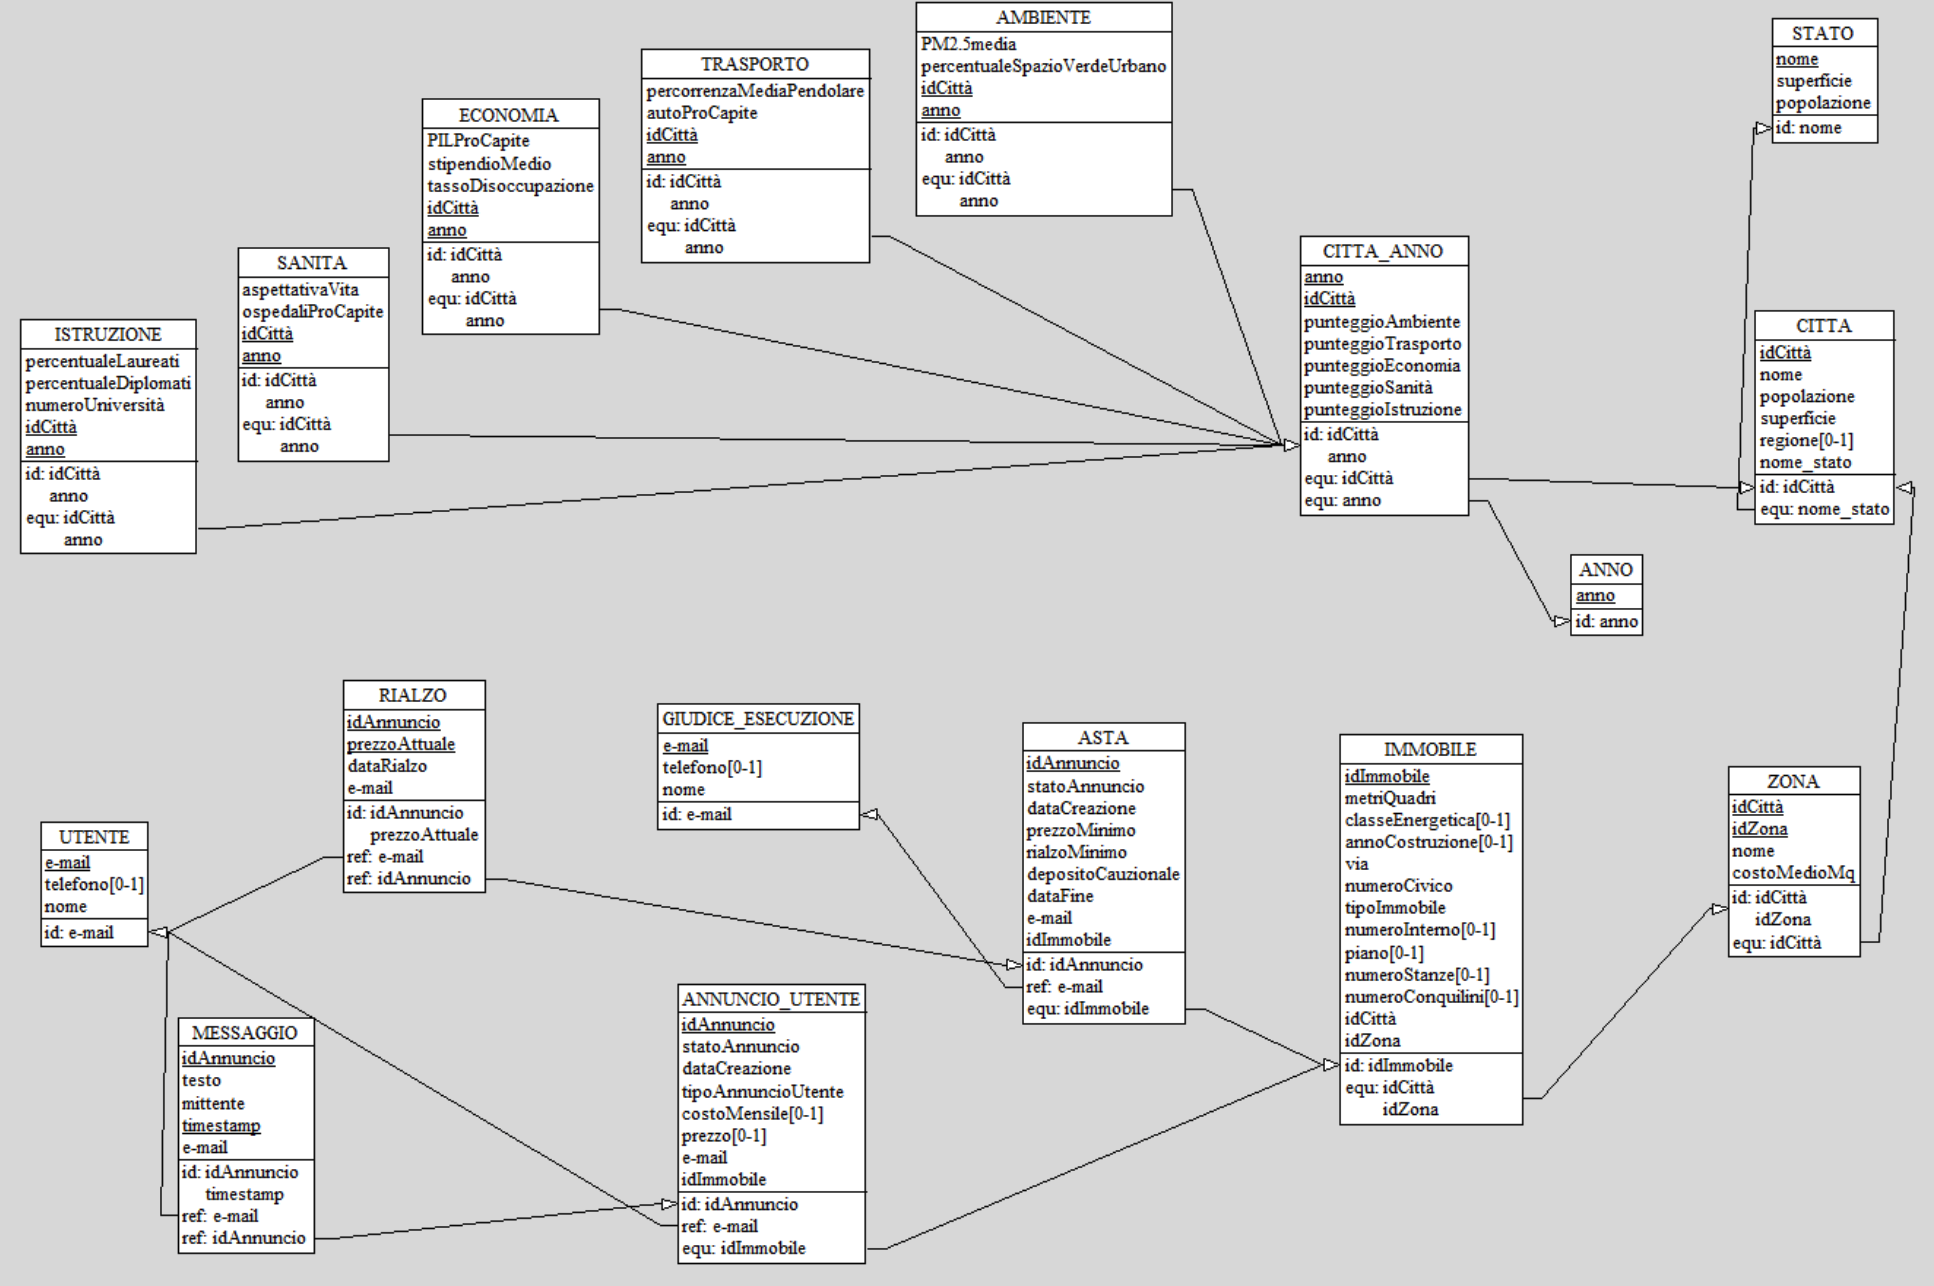
\includegraphics[width=\linewidth]{./images/relational_scheme.png}
                    \caption{Schema relazionale finale}
            \end{figure}
                
            \section{Traduzione delle operazioni in query SQL}

            \textbf{OP 1: Registrare un nuovo account} \\
            \texttt{
                \textcolor{blue}{INSERT INTO} utenti (e-mail, telefono, nome) \\
                \textcolor{blue}{VALUES} (?, ?, ?) \\
            } 
            
            \noindent
            \textbf{OP 2: Pubblicare un annuncio immobiliare (vendita o affitto)} \\
            \texttt{
                \textcolor{blue}{IF} (\textcolor{blue}{SELECT} \textcolor{blue}{COUNT}(*) \\
                \null\quad\quad\textcolor{blue}{FROM} immobili \\
                \null\quad\quad\textcolor{blue}{WHERE} via = ? \textcolor{blue}{AND} numeroCivico = ? \textcolor{blue}{AND} idCitta = ? > 0, \\
                \null\quad\quad TRUE, FALSE)  \\
            } \\
            Se tale condizione risulta soddisfatta, procediamo all'inizializzazione di \textit{annuncio\_utente} con i
            parametri appena trovati. Se non dovesse essere soddisfatta, vengono inseriti i dati di input. 
            In maniera analoga viene eseguita la query di inserimento di aste da parte dei giudici \\ \\
            \texttt{
                \textcolor{blue}{INSERT INTO} annunci\_utente (idAnnuncio, idImmobile, email, statoAnnuncio, dataCreazione, tipoAnnuncioUtente, costoMensile, prezzo) \\
                \textcolor{blue}{VALUES} (?, ?, ?, ?, ?, ?, ?, ?) \\
            }

            \noindent
            \textbf{OP 3: Visualizzare annunci immobiliari attivi di una città in ordine cronologico} \\
            \texttt{
                \textcolor{blue}{SELECT} * \\
                \textcolor{blue}{FROM} (immobili I \textcolor{blue}{JOIN} annunci\_utente A \textcolor{blue}{ON} (A.idImmobile = I.idImmobile)) \textcolor{blue}{JOIN} zone Z \textcolor{blue}{ON} (I.idZona = Z.idZona \textcolor{blue}{AND} Z.idCitta = ? \textcolor{blue}{AND} A.statoAnnuncio = 'Attivo') \\
                \textcolor{blue}{ORDER BY} A.dataCreazione  \textcolor{blue}{DESC} \\
            }

            \noindent
            \textbf{OP 4: Suddividere gli annunci in vendita, affitto o asta all’interno di una città} \\
            \texttt{
                \textcolor{blue}{SELECT} * \\
                \textcolor{blue}{FROM} (immobili I \textcolor{blue}{JOIN} annunci\_utente A \textcolor{blue}{ON} (A.idImmobile = I.idImmobile)) \textcolor{blue}{JOIN} zone Z \textcolor{blue}{ON} (I.idZona = Z.idZona \textcolor{blue}{AND} Z.idCitta = ? \textcolor{blue}{AND} A.statoAnnuncio = 'Attivo' \textcolor{blue}{AND} A.tipoAnnuncioUtente = ?) \\
                \textcolor{blue}{ORDER BY} A.dataCreazione  \textcolor{blue}{DESC} \\
            }
            \\
            Similmente vengono proiettate le aste attive in una data città in ordine di creazione decrescente.\\

            \noindent
            \textbf{OP 5: Ordinare gli annunci in base a particolari filtri sull'immobile (e.g. metratura, tipoImmobile)} \\
            AGGIUNGERE CASO ASTE \\
            \texttt{
                \textcolor{blue}{SELECT} * \\
                \textcolor{blue}{FROM} immobili I \textcolor{blue}{JOIN} annunci\_utente A \textcolor{blue}{ON} (I.idImmobile = A.idImmobile \textcolor{blue}{AND} A.statoAnnuncio = 'Attivo' \textcolor{blue}{AND} I.tipoImmobile = ?) \\
                \textcolor{blue}{WHERE} \textcolor{blue}{EXISTS} (\textcolor{blue}{SELECT} * \\
                    \null\qquad\qquad\qquad\quad\textcolor{blue}{FROM} zone Z, citta C \\
                    \null\qquad\qquad\qquad\quad\textcolor{blue}{WHERE} C.idCitta = ? \\
                    \null\qquad\qquad\qquad\quad\textcolor{blue}{AND} Z.idCitta= C.idCitta \\
                    \null\qquad\qquad\qquad\quad\textcolor{blue}{AND} Z.idZona = I.idZona) \\
            }

            \noindent
            \textbf{OP 6: Filtrare gli annunci per zona} \\
            AGGIUNGERE CASO ASTE \\
            \texttt{
                \textcolor{blue}{SELECT} * \\
                \textcolor{blue}{FROM} immobili I \textcolor{blue}{JOIN} annunci\_utente A \textcolor{blue}{ON} (I.idImmobile = A.idImmobile \\
                \textcolor{blue}{AND} A.statoAnnuncio = "Attivo" \textcolor{blue}{AND} I.idZona = ?) \\
                \textcolor{blue}{ORDER BY} dataCreazione   \textcolor{blue}{DESC} \\
            }

            \noindent
            \textbf{OP 7: Ordinare gli annunci di affitto per costo mensile} \\
            \texttt{
                \textcolor{blue}{SELECT} * \\
                \textcolor{blue}{FROM} immobili I \textcolor{blue}{JOIN} annunci\_utente A \textcolor{blue}{ON} (I.idImmobile = A.idImmobile \textcolor{blue}{AND} A.statoAnnuncio = 'Attivo' \textcolor{blue}{AND} A.tipoAnnuncioUtente = 'Affitto') \\
                \textcolor{blue}{WHERE EXISTS} (\textcolor{blue}{SELECT} * \\
                    \null\qquad\qquad\qquad\quad\textcolor{blue}{FROM} zone Z, citta C \\
                    \null\qquad\qquad\qquad\quad\textcolor{blue}{WHERE} C.idCitta = ? \\
                    \null\qquad\qquad\qquad\quad\textcolor{blue}{AND} Z.idCitta = C.idCitta \\
                    \null\qquad\qquad\qquad\quad\textcolor{blue}{AND} Z.idZona = I.idZona) \\
                \textcolor{blue}{ORDER BY} A.costoMensiile \textcolor{blue}{DESC} \\
            }
            
            \noindent
            \textbf{OP 8: Mostrare aste attive in una città} \\
            \texttt{
                \textcolor{blue}{SELECT} * \\
                \textcolor{blue}{FROM} (immobili I \textcolor{blue}{JOIN} Aste A \\ 
                \textcolor{blue}{ON} (A.idImmobile = I.idImmobile)) \textcolor{blue}{JOIN} Zone Z \\ 
                \textcolor{blue}{ON} (I.idZona = I.idZona \textcolor{blue}{AND} Z.idCitta = ? \textcolor{blue}{AND} A.dataFine > \textcolor{blue}{NOW()}) \\
                \textcolor{blue}{ORDER BY} A.DataCreazione  \textcolor{blue}{DESC} \\
            }
            
            \noindent
            \textbf{OP 9: Ordinare le aste per prezzo attuale crescente} \\
            \texttt{
                \textcolor{blue}{SELECT} idAnnuncio, \textcolor{blue}{IF}(( \textcolor{blue}{SELECT COUNT}(*) \\
                    \null\qquad\qquad\qquad\qquad\qquad\qquad \textcolor{blue}{FROM} rialzi R \\
                    \null\qquad\qquad\qquad\qquad\qquad\qquad \textcolor{blue}{WHERE} R.idAnnuncio = idAnnuncio) == 0, \\
                    \null\qquad\qquad\qquad\qquad\qquad\qquad prezzoMinimo, \\
                    \null\qquad\qquad\qquad\qquad\qquad\qquad (\textcolor{blue}{DECLARE} prezzoMassimo float; \\
                    \null\qquad\qquad\qquad\qquad\qquad\qquad \textcolor{blue}{SELECT TOP}(1) prezzoAttuale \\
                    \null\qquad\qquad\qquad\qquad\qquad\qquad \textcolor{blue}{INTO} prezzoMassimo \\
                    \null\qquad\qquad\qquad\qquad\qquad\qquad \textcolor{blue}{FROM} rialzi R \\
                    \null\qquad\qquad\qquad\qquad\qquad\qquad \textcolor{blue}{WHERE} R.idAnnuncio = idAnnuncio \\
                    \null\qquad\qquad\qquad\qquad\qquad\qquad \textcolor{blue}{ORDER BY} prezzoAttuale \textcolor{blue}{DESC}; \\
                    \null\qquad\qquad\qquad\qquad\qquad\qquad prezzoMassimo)) \\
                \textcolor{blue}{FROM} aste \\
                \textcolor{blue}{WHERE} dataFine > \textcolor{blue}{NOW()} \\
            }

            \noindent
            \textbf{OP 10: Effettuare un rialzo all’interno di un’asta (controllando la sua validità)} \\
            \texttt{
                \textcolor{blue}{IF} ((\textcolor{blue}{SELECT MAX}(prezzoAttuale) \\
                    \null\qquad \textcolor{blue}{FROM} rialzi \\
                    \null\qquad \textcolor{blue}{WHERE} idAnnuncio = ?) <= ? - (\textcolor{blue}{SELECT} rialzoMinimo \\
                        \null\qquad\qquad\qquad\qquad\qquad\qquad\qquad\qquad\qquad \textcolor{blue}{FROM} aste \\
                        \null\qquad\qquad\qquad\qquad\qquad\qquad\qquad\qquad\qquad \textcolor{blue}{WHERE} idAnnuncio = ?), \\
                    \null\qquad \textcolor{blue}{INSERT INTO} rialzi(prezzoAttuale, email, idAnnuncio, dataRialzo) \\
                    \null\qquad \textcolor{blue}{VALUES}(?, ?, ?, ?), \\ 
                    \null\qquad \textcolor{blue}{NULL}) \\
            }       
            
            \noindent
            \textbf{OP 11: Contattare un utente in merito ad un annuncio creato} \\
            \texttt{
                \textcolor{blue}{INSERT INTO} messaggi (timestamp, email, idAnnuncio, testo, mittente) \\
                \textcolor{blue}{VALUES} (\textcolor{blue}{NOW()}, ?, ?, ?, ?) \\
            } 

            \noindent
            \textbf{OP 12: Ricostruire una conversazione tra due utenti} \\
            \texttt{
                \textcolor{blue}{SELECT} testo, mittente, timestamp \\
                \textcolor{blue}{FROM} messaggi \\
                \textcolor{blue}{WHERE} email = ? \\
                \textcolor{blue}{AND} idAnnuncio = ? \\
                \textcolor{blue}{ORDER BY} timestamp \\
            }

            \noindent
            \textbf{OP 13: Andamento del prezzo di un immobile in funzione del tempo} \\
            \texttt{
                \textcolor{blue}{SELECT} dataCreazione, prezzo, costoMensile \\
                \textcolor{blue}{FROM} annunci\_utente \\
                \textcolor{blue}{WHERE} idImmobile = ? \\
                \textcolor{blue}{ORDER BY} dataCreazione \textcolor{blue}{DESC} \\
            }
            
            \noindent
            \textbf{OP 14: Comparare il prezzo di un immobile al mq con quello degli immobili nella stessa zona} \\
            \texttt{
                \textcolor{blue}{SELECT} ((prezzo/metriQuadri)-costoMedioMq) * 100/costoMedioMq \\
                \textcolor{blue}{FROM} (immobili I \textcolor{blue}{JOIN} annunci\_Utente A  \\
                \textcolor{blue}{ON} (A.idImmobile = I.idImmobile)) \textcolor{blue}{JOIN} Zone Z \\
                \textcolor{blue}{ON} (I.idZona = Z.idZona) \\
                \textcolor{blue}{WHERE} idImmobile = ? \textcolor{blue}{AND} statoAnnuncio = 'Attivo' \\
            }
            
            \noindent
            \textbf{OP 15: Comparare il prezzo di un immobile al mq con quello degli immobili nella stessa città} \\
            \texttt{
                \textcolor{blue}{SET} @costoMedioMqCitta = (\textcolor{blue}{SELECT SUM}(costoMedioMq*numeroImmobili) \\
                    \null\qquad\qquad\qquad\qquad\qquad\qquad\quad\textcolor{blue}{FROM} zone \\
                    \null\qquad\qquad\qquad\qquad\qquad\qquad\quad\textcolor{blue}{WHERE} idCitta = ?) / \textcolor{blue}{SELECT SUM}(numeroImmobili) \\
                        \null\qquad\qquad\qquad\qquad\qquad\qquad\qquad\qquad\qquad\qquad\qquad\qquad\textcolor{blue}{FROM} zone  \\
                        \null\qquad\qquad\qquad\qquad\qquad\qquad\qquad\qquad\qquad\qquad\qquad\qquad\textcolor{blue}{WHERE} idCitta = ? \\
                \textcolor{blue}{SELECT} ((prezzo/metriQuadri)-@costoMedioMqCitta) * 100/@costoMedioMqCitta \\
                \textcolor{blue}{FROM} (immobili I \textcolor{blue}{JOIN} annunci\_Utente A  \\
                \textcolor{blue}{ON} (A.idImmobile = I.idImmobile)) \textcolor{blue}{JOIN} Zone Z \\
                \textcolor{blue}{ON} (I.idZona = Z.idZona) \textcolor{blue}{JOIN} Città C \\
                \textcolor{blue}{ON} (Z.idCittà = C.idCittà) \\
                \textcolor{blue}{WHERE} idImmobile = ? \textcolor{blue}{AND} statoAnnuncio = 'Attivo' \\
            }

            \noindent
            \textbf{OP 16: Comparare il prezzo medio al mq di una zona con quello della città} \\
            \texttt{
                \textcolor{blue}{SELECT} * \\
                \textcolor{blue}{FROM}  \\
                \textcolor{blue}{SELECT} idZona, (costoMedioMq-\textcolor{blue}{SUM}(costoMedioMq * numeroImmobili)/ \\
                \textcolor{blue}{SUM}(numeroImmobili)) * 100 / \textcolor{blue}{SUM}(costoMedioMq * numeroImmobili)/ \\
                \textcolor{blue}{SUM}(numeroImmobili) \\
                \textcolor{blue}{FROM} zone \\
                \textcolor{blue}{WHERE} idCitta = ? \textcolor{blue}{AS} percZonaCitta\\
                \textcolor{blue}{WHERE} percZonaCitta.idZona = ? \\
            }

            \noindent
            \textbf{OP 17: Ordinare le zone di una città per costo medio al mq} \\
            \texttt{
                \textcolor{blue}{SELECT} * \\
                \textcolor{blue}{FROM} zone \\
                \textcolor{blue}{WHERE} idCitta = ? \\
                \textcolor{blue}{ORDER BY} costoMedioMq \textcolor{blue}{DESC} \\
            }

            \noindent
            \textbf{OP 18: Stilare una top 5 città per una o più categorie} \\
            \texttt{
                \textcolor{blue}{SELECT TOP}(5) \textcolor{blue}{WITH TIES} \\
                \textcolor{blue}{FROM} citta\_anni A\\
                \textcolor{blue}{WHERE} A.anno = ? \\
                \textcolor{blue}{ORDER BY} A.punteggioAmbiente*?+ \\
                A.punteggioTrasporto*?+A.punteggioEconomia*?+ \\
                A.punteggioSanità*?+A.punteggioIstruzione*? \textcolor{blue}{DESC} \\
            }
            
            \noindent
            \textbf{OP 19: Classificare città in base all’evoluzione in una o più categorie rispetto all’anno precedente} \\
            \texttt{
                \textcolor{blue}{SELECT} punteggioAmbiente+punteggioTrasporto+punteggioEconomia+punteggioSanita+punteggioIstruzione AS punteggioCitta, anno \\
                \textcolor{blue}{FROM} citta\_anni \\
                \textcolor{blue}{WHERE} idCitta = ? \textcolor{blue}{AND} anno = ? \\
            }
            
            \noindent
            \textbf{OP 20: Ordinare le città in base a valori specifici di una o più categorie} \\
            \texttt{
                \textcolor{blue}{SELECT} A.percentualeSpazioVerdeUrbano, C.nome, C.anno, C.idCitta \\
                \textcolor{blue}{FROM} ambiente A, citta\_anni C \\
                \textcolor{blue}{WHERE} A.hashAmbiente = C.hashAmbiente  \\
                \textcolor{blue}{AND} C.anno = ? \\
                \textcolor{blue}{ORDER BY} A.percentualeSpazioVerdeUrbano \textcolor{blue}{DESC} \\
            }
            
            \noindent
            \textbf{OP 21: Calcolare performance di uno stato in una o più categorie (da ogni città)} \\
            \texttt{
                \textcolor{blue}{SELECT AVG} (A.punteggio*) \\
                \textcolor{blue}{FROM} (stati S \textcolor{blue}{JOIN} citta C \\
                \textcolor{blue}{ON} (S.nome = C.nomeStato)) \\
                \textcolor{blue}{JOIN} citta\_anni A \\
                \textcolor{blue}{ON} (A.idCitta = C.idCitta \textcolor{blue}{AND} anno = ?) \\
                \textcolor{blue}{WHERE} C.nomeStato = ? \\
            }

            \noindent
            \textbf{OP 22: Aggiornamento annuale dei punteggi di una città (dati i campi delle categorie)} \\
            \texttt{
                newHashAmbiente = \textcolor{blue}{CAST}(pm25media*10 \textcolor{blue}{AS} int)*1001 + \textcolor{blue}{CAST}(percentualeSpazioVerdeUrbano*10 \textcolor{blue}{AS} int) \\ \\
                \textcolor{blue}{IF} ((SELECT COUNT(hashAmbiente) \\
                \textcolor{blue}{FROM} ambiente \\
                \textcolor{blue}{WHERE} hashAmbiente = newHashAmbiente) > 0,  \\
                \textcolor{blue}{NULL},  \\
                \textcolor{blue}{INSERT INTO} ambiente(hashAmbiente, pm25media, percentualeSpazioVerdeUrbano) \\
                \textcolor{blue}{VALUES} (newHashAmbiente, ?, ?)) \\
                \textcolor{blue}{INSERT INTO} citta\_anni(punteggioAmbiente, newHashAmbiente) \\
            }

        \chapter{Progettazione dell'applicazione}
            
    	\section{Descrizione dell'architettura dell'applicazione realizzata}
        	asdasd
 
\end{document}